% ============================================================
%  Small Paper --- ASR (Advances in Space Research)
%  Title: Physics-Aware Multi-Objective Scheduling for Agile SAR
%         Satellites: Balancing Profit, NESZ, and Geometric Resolution
% ============================================================
\documentclass[preprint,12pt,authoryear]{elsarticle}
% ── Packages ──
\usepackage{amsmath,amssymb,amsfonts}
\usepackage{booktabs}
\usepackage{caption}
\captionsetup{justification=centering}
\usepackage{subcaption}
\usepackage{multirow}
\usepackage{enumitem}
\usepackage{float}
\usepackage{hyperref}
\graphicspath{{figures/}}
% ── Journal ──
\journal{Advances in Space Research}
% ── Metadata ──
\begin{document}
\begin{frontmatter}
\title{Physics-Aware Multi-Objective Scheduling for an Agile SAR Satellite: Balancing Profit, NESZ, and Geometric Resolution}
\author{LIU Shuhao}
\ead{liushuhao@hrbeu.edu.cn}
\affiliation{organization={College of Intelligent Systems Science and Engineering, Harbin Engineering University},
            addressline={145 Nantong Street, Nangang District},
            city={Harbin},
            postcode={150001},
            country={China}}
% ============================================================
%  ABSTRACT (~200 words)
% ============================================================
\begin{abstract}
In agile SAR scheduling, observation timing determines imaging quality
through radar-specific geometric and radiometric effects. We present a
physics-aware multi-objective formulation of single-satellite Stripmap
scheduling that optimizes coverage profit, geometric resolution, and
noise-equivalent sigma-zero (NESZ) radiometric quality simultaneously within
a non-dominated sorting genetic algorithm III (NSGA-III) framework, and we
characterize how the value of physical quality objectives depends on target
density. Across 200 scenarios spanning densities 20--500, the benefit of
multi-objective optimization is scale-dependent: at sparse density,
re-optimizing observation times yields a $+34\%$ gain in geometric quality
at a $14\%$ coverage cost, and the three-objective variant attains
radiometric quality $+40\%$ above the greedy-coverage baseline at a $15\%$
coverage cost; under a matched knee-point rule the third objective
contributes a controlled $+4.9\%$ radiometric margin over the two-objective
variant, and this margin only materializes when the selected knee point is
radiometric-aware. A single-point squint-minimized heuristic reaches
comparable radiometric quality only at roughly half the coverage of the
greedy baseline, so the multi-objective advantage is the small coverage
price paid for the quality gain;
at high densities ($N \geq 300$), the multi-objective solvers
converge to the greedy coverage anchor and marginal quality gains fall below
$2\%$. This convergence is conditional on greedy hot-start initialization. The third
(radiometric) objective remains density-dependent rather than redundant:
the geometric--radiometric trade-off is mild in raw visibility geometry
($r \approx -0.36$) but is actively exploited under sparse-density
scheduling ($r \approx -0.63$, matching the independent-angle null) and
collapses under coverage pressure at high density ($r \approx -0.15$). These results establish an empirical, conditional saturation
regime that delimits when physics-aware multi-objective scheduling benefits
single-satellite SAR operations.
\end{abstract}
\begin{keyword}
agile SAR \sep satellite scheduling \sep multi-objective optimization \sep NSGA-III \sep noise-equivalent sigma zero (NESZ) \sep geometric resolution
\end{keyword}
\end{frontmatter}
% ============================================================
%  1. INTRODUCTION (~900 words)
% ============================================================
\section{Introduction}
\label{sec:introduction}
Agile Earth-observation satellites equipped with Synthetic Aperture Radar (SAR)
are increasingly central to time-critical monitoring missions, from disaster response
to maritime surveillance.
Their agility (the ability to slew the antenna beam away from the nadir track)
enables a single satellite to image far more targets per orbit than a fixed-pointing
platform \citep{Curlander1991}.
This flexibility, however, transforms scheduling from a simple feasibility check
into a combinatorial optimization problem: for $N$ targets each with a finite
visibility window, the scheduler must select a subset and assign observation times
that satisfy attitude transition constraints while maximizing some measure of
mission value.
Throughout this paper, ``single-pass'' denotes a single satellite operating over a two-orbit scheduling
horizon ($\sim 200$ min, at most one observation per target), not a single overflight.
In conventional satellite scheduling, observation quality is commonly
represented as a fixed attribute of each pre-computed opportunity rather than
a quantity that varies with the selected acquisition time. The scheduling
problem therefore reduces to maximizing the number or priority-weighted
sum of observed targets subject to temporal feasibility.
This assumption underpins most existing satellite scheduling work,
from mixed-integer programming formulations to deep reinforcement learning
approaches \citep{Chen2025NeuralPriority}.

SAR imaging departs fundamentally from this assumption when the scheduler can choose the acquisition time, because image quality depends on the radar geometry at the moment of acquisition:
the ground-range resolution degrades with incidence angle ($\rho_{\text{rg}} \propto 1/\sin\theta$),
the azimuth resolution broadens with squint angle ($\rho_{\text{az}} \propto 1/\cos\psi_{\text{sq}}$),
and the radiometric sensitivity (Noise-Equivalent Sigma Zero, NESZ) deteriorates
with slant range as $R^3$ \citep{Cumming2005}.
When the scheduler can choose \emph{when} within a visibility window to observe
each target (the defining feature of agile satellites), it simultaneously
chooses the imaging quality at which each target is acquired.
Despite this tight coupling between scheduling and imaging physics,
with few exceptions \citep{Kramer2025SARVis}, existing
agile SAR scheduling methods either reduce SAR to a coverage-only objective
or apply post hoc quality checks on schedules produced by
coverage-maximizing solvers.
Few approaches treat physical quality dimensions as primary optimization
objectives in the SAR domain.

The problem is NP-hard by reduction from the Orienteering Problem with
Time-Dependent Profits \citep{Peng2019Orienteering}, precluding
polynomial-time exact algorithms for all but the smallest instances.
The SAR literature has well-established models for NESZ and geometric resolution
as functions of observation geometry \citep{Curlander1991,Cumming2005}, and
the multi-objective optimization literature provides mature frameworks such
as the Non-dominated Sorting Genetic Algorithm III (NSGA-III) \citep{Deb2014} for handling three or more objectives simultaneously.
Yet direct integration of these three elements (SAR physical modeling,
multi-objective evolutionary algorithms (MOEAs), and satellite scheduling)
remains limited. We therefore formulate SAR scheduling with separate,
physics-derived geometric and radiometric quality objectives within a MOEA
framework.

We formulate a three-objective agile SAR scheduling problem in which the
scheduler optimizes (1) total coverage profit, (2) mean geometric image quality
(ground-range and azimuth resolution), and (3) mean NESZ radiometric quality
simultaneously (denoted $f_1^*$, $f_2$, and $f_3$ below,
\S~\ref{sec:objective-functions}).
We compare five solver configurations spanning the methodological spectrum: two greedy
heuristics (one profit-only baseline and one squint-minimized variant), a
single-objective genetic algorithm with greedy hot-start (GA-P-BL, a control
that returns the greedy schedule whenever it fails to improve profit, so it
is never worse than G-BL and is numerically identical to G-BL in 199 of 200
scenarios), and two NSGA-III
variants with two and three objectives.
The solvers are evaluated on 200 systematically varied scenarios across four
density classes ($N = 20$ to $N = 500$).
Our results show a scale-dependent saturation, not a uniform solver advantage.
In sparse scenarios, multi-objective optimization can extract substantial
radiometric gains (MOEA-3 raises $f_3$ by $+40\%$
relative to G-BL at a $15\%$ coverage cost) alongside modest geometric
gains (MOEA-2, $+34\%$ in $f_2$ at a $14\%$ coverage cost; the best-coverage front point gives $+12.5\%$ in $f_2$).
Under a matched radiometric-aware knee rule, the third objective accounts for
a controlled $+4.9\%$ of this $f_3$ margin; the margin does not appear under a
radiometric-blind selection rule, so it is conditional on the knee-point
choice. The single-point squint-minimized heuristic (G-SM) attains slightly
higher $f_3$ than MOEA-3 in sparse scenarios but only at roughly half the
coverage of G-BL ($f_1^* \approx 0.51$), so the multi-objective advantage is
the small coverage price paid for the quality gain.
In dense scenarios, the multi-objective advantage diminishes to negligible
levels: greedy methods attain the tested family's coverage reference, and the
squint-minimized heuristic offers competitive radiometric quality. This
convergence is conditional on the G-BL hot start
(\S~\ref{sec:robustness-calibration}), and the fronts are best-known NSGA-III
approximations rather than verified Pareto-optimal sets.
\S~\ref{sec:summary} provides a detailed synthesis of these findings.
The specific contributions of the paper are:
\begin{enumerate}[nosep]
    \item The discovery and analytical characterization of an empirical saturation
    regime for greedy-baseline-seeded (G-BL-seeded) multi-objective SAR quality
    optimization in the
    single-pass, single-satellite Stripmap setting under the tested
    configuration: solver convergence to lower-squint geometries attenuates the
    envelope-level conflict between geometric and radiometric quality while
    coverage pressure removes the room to trade objectives against each other
    (\S~\ref{sec:pareto-coupling}), not a physical identity between objectives,
    making the three-objective formulation indistinguishable in class means
    from the two-objective one at high densities under the tested search
    (a trace per-scenario radiometric advantage persists even at the densest class);
    \item A controlled ablation study (four objective-function variants over
    six scenario classes---four density classes plus two targeted robustness
    classes---totaling 300 scenarios per variant) and initialization controls
    (\S~\ref{sec:robustness-calibration}) showing that solver outcomes become
    invariant to the choice of physical objectives at high target densities,
    that coverage convergence is conditional on greedy-baseline (G-BL)
    hot-start initialization, and that the fronts are best-known NSGA-III
    approximations, not verified Pareto-optimal sets;
    \item An anchor-independent geometric-coupling baseline: the
    $f_2$--$f_3$ trade-off is mild within raw visibility geometry
    ($r \approx -0.36$, versus an independent-angle null of $r \approx
    -0.60$), is restored to the null strength in sparse schedules
    ($-0.63$) by squint-aware steering, and collapses to $-0.2$ to
    $-0.15$ at high density under coverage pressure, isolating
    where the third objective's value is lost to convergence rather than
    to a mathematical redundancy;
    \item The decomposition of SAR image quality into closed-form NESZ
    ($\propto R^3$) and geometric quality index ($\sin\theta\cos\psi_{\text{sq}}$,
    the dimensionless inverse of the ground pixel area since
    $\rho_{\text{rg}} \propto 1/\sin\theta$ and $\rho_{\text{az}} \propto 1/\cos\psi_{\text{sq}}$)
    objectives within an NSGA-III framework, distinct from the scalar
    visibility composite of \citet{Kramer2025SARVis} and
    the generic image-quality composite of \citet{Wei2025MONP}, using
    mean per-task quality metrics that decouple quality from the number of
    scheduled tasks. This formulation enables the systematic characterization
    of quality--coverage trade-offs across two greedy heuristics, a
    single-objective GA control, and two NSGA-III variants on four scale
    classes (200 scenarios).
\end{enumerate}
% ============================================================
%  2. RELATED WORK (~900 words)
% ============================================================
\section{Related Work}
We examine three lines of research that our study connects:
satellite scheduling (2.1), SAR physical quality modeling (2.2),
and multi-objective evolutionary optimization (2.3).
\subsection{Satellite Scheduling}
Satellite scheduling has been studied extensively in the Earth-observation
domain. The survey by \citet{Ferrari2025} catalogs over 200
publications spanning exact methods, heuristics, metaheuristics, and
learning-based approaches. Exact formulations based on mixed-integer linear
programming (MILP) achieve optimality on small instances but fail to scale
to operational problem sizes, motivating a broad family of heuristic and
metaheuristic alternatives including genetic algorithms, simulated annealing,
and tabu search~\citep{Wang2019MILP,Chen2019MILPMulti}.
The earliest formal treatments of agile satellite scheduling by
\citet{Lemaitre2002MultiSat} and
\citet{Bianchessi2007} established the
foundational problem structure of time-dependent transition
times between observations.
Recent work further generalizes these methods to agile satellites, where
the freedom to choose observation start times within each visibility window
is exploited to pack more observations into a single orbit~\citep{Peng2019Orienteering,Chen2024LearnConstruct}.
A parallel line of research has pursued learning-based and hybrid approaches
for satellite scheduling. \citet{Liu2024TwoStageDRL} and
\citet{Zhou2025TwoPhase} apply deep reinforcement learning to
agile optical satellite scheduling, while \citet{Jacquet2024GNN}
combine graph neural networks with Monte Carlo tree search for the same domain.
\citet{Wang2026Lagrangian} propose a Lagrangian relaxation-based
heuristic for multi-satellite mission planning.
\citet{Caleiras2026SuperAgile} formulate super-agile
satellite scheduling as a constraint programming problem, capturing
the time-dependent transition constraints characteristic of super-agile platforms.
\citet{Herrmann2023} apply RL to on-board AEOS scheduling, maximizing target collection reward without imaging quality as an objective.
\citet{Wu2026WhaleHighDensity} address high-target-density AEOS scheduling with an improved whale optimization algorithm, reporting convergence challenges that echo the density-driven constraint tightening we analyze in \S~\ref{sec:scale-sensitivity}.
Despite their methodological diversity, most prior
works treat quality as a fixed property determined at observation-window
generation. In contrast, SAR imaging quality varies continuously with acquisition
geometry and is directly optimizable within the scheduling window. \citet{Chang2022Gaofen}
propose early MOEAs for SAR satellite scheduling that combine an adaptive large
neighborhood search with NSGA-II and NSGA-III selection; their three-objective
model (ground-target loss rate, invalid observations, and sensor-activation
count) targets operational metrics --- the closest prior work to ours --- but
it omits imaging quality dimensions. \citet{Wei2025MONP}
introduce a neural-policy-guided MOEA that incorporates a composite image
quality score as an optimization objective. \citet{Kramer2025SARVis}
schedule SAR constellation observations with a hybrid metaheuristic using a
weighted visibility--performance composite, embedding a SAR-quality proxy in
the scheduler, and \citet{Yao2024Bilevel}
develop a bilevel evolutionary algorithm for multi-satellite scheduling
that separates task allocation from detailed observation planning.
\citet{ChangZhou2025Memetic} formulate agile Earth-observation scheduling
with a bi-objective image-quality-loss/energy model in which quality enters as
an attitude-angle proxy attached to each observation opportunity, and
\citet{Wu2019NSGA3Formation} apply NSGA-III to satellite-formation imaging
scheduling with coverage- and timeliness-type objectives; in this
literature imaging quality is a scalar attribute or coarse proxy rather than a
decomposed physical objective.
The common limitation of this prior work is that SAR physical quality
metrics---noise-equivalent sigma zero (NESZ), azimuth resolution,
ground-range resolution---are either absent or approximated by coarse
proxies (e.g., penalizing extreme off-nadir angles). To our knowledge,
no existing SAR scheduling method treats continuous, physics-derived
quality functions as decomposed optimization objectives in their own
right: the closest approaches embed aggregated quality
proxies rather than separate geometric and radiometric objectives.
\subsection{SAR Physical Quality Modeling}
The SAR remote sensing literature provides well-established analytical
models linking observation geometry to image quality.
\citet{Curlander1991}, \citet{Cumming2005}, and \citet{Moreira2026} give detailed treatments
of SAR physics, including the two quality dimensions relevant to scheduling:
geometric resolution and radiometric sensitivity.
Geometric resolution decomposes into ground-range resolution
$\rho_{\text{rg}} = c / (2B \sin\theta)$, where $c$ is the speed of light,
$B$ the radar bandwidth, and $\theta$ the incidence angle, and azimuth
resolution $\rho_{\text{az}} = D / (2 \cos\psi_{\text{sq}})$, where $D$
is the antenna length and $\psi_{\text{sq}}$ the squint angle. In
operational SAR, amplitude weighting widens $\rho_{\text{az}}$ by
10--20\%~\citep{Curlander1991}, but since this is platform-constant, the
unweighted form preserves the relative ordering for optimization.
The two resolution components respond oppositely to departure from the
zero-Doppler geometry ($\psi_{\text{sq}} = 0$, $\theta$ minimal):
$\rho_{\text{az}}$ worsens as $|\psi_{\text{sq}}|$ grows, whereas
$\rho_{\text{rg}}$ is coarsest at the minimal incidence of closest approach
and improves as $\theta$ rises away from it---the origin of the $\theta$-axis
trade-off formalized in \S~\ref{sec:objective-functions}. Radiometric sensitivity,
measured by the Noise-Equivalent Sigma Zero (NESZ), deteriorates with the
cube of slant range: $\text{NESZ} \propto R^3$ for Stripmap SAR after azimuth compression
gain~\citep{Curlander1991,Moreira2026}. The specific range decomposition and
ordering-index approximation used in this work are derived in
\S~\ref{sec:objective-functions}.
These quality models are routinely used in SAR system design but their use in
scheduling remains limited to post hoc validation of fixed
observation plans~\citep{KramerMiller2024} or binary feasibility filtering
at the observation-window level~\citep{QualityScreening2026}. The
scheduling literature and the SAR quality modeling literature have
developed in parallel: schedulers treat quality as a constraint, while
SAR engineers compute quality after the schedule is fixed. Our study
connects these two domains by embedding continuous quality functions
directly into the optimization objective space.
\subsection{Multi-Objective Evolutionary Optimization}
Multi-objective evolutionary algorithms (MOEAs) are a standard toolkit
for problems with competing objectives. The NSGA-III algorithm
\citep{Deb2014} extends the NSGA-II framework \citep{Deb2002NSGA2} to many-objective problems
through reference-point-based diversity preservation.
The hypervolume (HV) indicator is widely used for comparing Pareto fronts
\citep{Zitzler1999HV}, but its sensitivity to frontier cardinality creates
interpretational challenges when mixing single-objective and multi-objective
solvers, a methodological issue we address in \S~\ref{sec:pareto-coupling}.
To our knowledge, MOEAs have not been applied to SAR scheduling with
physical quality objectives; the closest work
uses single-objective optimization with post hoc quality evaluation.
Our NSGA-III formulation makes these trade-offs explicit by placing
coverage profit, geometric quality, and radiometric quality in a unified
multi-objective framework.
% ============================================================
%  3. PROBLEM FORMULATION (~1100 words)
% ============================================================
\section{Problem Formulation}
% ── 3.1 System Model ──
\subsection{System Model}\label{sec:system-model}
% Satellite orbit, task set, visibility windows
% Key parameters: H, ω_max, τ_settle
% Decision variables: x_i (selection), t_i (start time)
We consider a single agile SAR satellite in a circular orbit at altitude $H$,
operating in Stripmap mode, which provides the widest continuous swath with
uniform quality and analytically tractable NESZ and resolution expressions
\citep{Curlander1991}.
A problem instance $\mathcal{I} = (\mathcal{T}, \mathcal{P}, \mathcal{O})$ consists of
a set of $N$ ground targets $\mathcal{T}$, a satellite platform $\mathcal{P}$,
and a SAR imaging model $\mathcal{O}$.
\paragraph{Task Set.}
Each task $i \in \{1,\ldots,N\}$ is specified by its geographic coordinates
$\mathbf{r}_i = (\phi_i, \lambda_i)$, a priority weight $p_i \in \mathbb{R}^+$, a visibility window
$\mathcal{W}_i = [a_i, b_i]$ during which the satellite can observe the target,
and a fixed observation duration $d_i$.
\paragraph{Satellite Platform.}
The satellite is characterized by its maximum slew rate $\omega_{\max}$ (a
conservative single-axis bound on three-axis attitude maneuvers), settling
time $\tau_{\text{settle}}$ after each maneuver, per-orbit energy budget
$E_{\max}$ and memory budget $M_{\max}$, and per-observation energy $e_i$
and memory $m_i$ consumption.
\paragraph{SAR Observables.}
Given an observation time $t_i$, the satellite-to-target line-of-sight (LOS)
vector $\mathbf{l}(t_i)$ in the Local-Vertical Local-Horizontal (LVLH) frame
is fully determined by the satellite's orbital state.
From $\mathbf{l}(t_i)$ we derive four geometric quantities deterministically:
slant range $R = |\mathbf{l}|$, off-nadir angle $\xi = \arctan2(\sqrt{l_x^2+l_y^2},\, l_z)$,
incidence angle $\theta$ (via the Earth-curvature-corrected mapping
$\theta = \arcsin\big(\frac{R_e+H}{R_e}\sin\xi\big)$ where $R_e$ is Earth's mean radius), and
squint angle $\psi_{\text{sq}} = \arcsin(|l_x| / R)$ (LVLH $x$-axis
along-track, $z$-axis nadir-pointing), defined as the
angular deviation of the LOS vector from the zero-Doppler plane
\citep{Curlander1991}.
For the objectives we also use the elevation-plane incidence angle
$\theta_{\text{elev}}$, defined through the identity
$\cos\theta_{\text{elev}} = \cos\xi / \cos\psi_{\text{sq}}$
(i.e., the incidence angle of the LOS projection onto the cross-track plane);
this isolates the cross-track ground-range geometry from the along-track
squint contribution. $\theta_{\text{elev}}$ is the satellite-centered
elevation-plane angle; it differs from the target-side incidence angle of
\S\ref{sec:system-model} by a few degrees due to Earth curvature at
these orbital altitudes, but it preserves the cross-track ordering of
candidate views, so using it in the geometric-quality objective of
\S~\ref{sec:objective-functions} is ordering-consistent.
A critical property is that \emph{all} quality-relevant geometry
is a deterministic function of the single decision $t_i$.
\paragraph{Decision Variables.}
A schedule consists of a task selection vector $\mathbf{x} \in \{0,1\}^N$,
an ordered sequence $S = (s_1,\ldots,s_m)$ of the $m$ selected tasks, and
a vector of observation start times $\mathbf{t} = (t_{s_1},\ldots,t_{s_m})$.
All geometric parameters ($\theta_i$, $\psi_{\text{sq},i}$, $R_i$) are
\emph{derived} from $t_i$ rather than independent decision variables.
% ── 3.2 Objective Functions ──
\subsection{Objective Functions}\label{sec:objective-functions}
We formulate a three-objective optimization problem that captures the
tension between scheduling throughput and SAR-specific imaging quality.
All quality objectives use the \emph{mean} over scheduled tasks, making
them independent of the number of scheduled tasks $m = |\mathcal{S}|$
and thereby producing a genuine ``quantity versus quality'' Pareto trade-off.
\paragraph{Objective 1: Coverage Profit.}
The normalized coverage profit (Eq.~\ref{eq:f1}) is defined relative to the greedy baseline
\begin{equation}
f_1^* = \frac{1}{f_1^{\text{G-BL}}} \sum_{i \in \mathcal{S}} p_i
\label{eq:f1}
\end{equation}
where $f_1^{\text{G-BL}}$ is the profit achieved by the profit-only greedy
scheduler (G-BL, \S~\ref{sec:gbl}) on the same scenario.
Normalization by G-BL rather than GA-P-BL is conservative for the
MOEA coverage deficit: GA-P-BL output is identical to G-BL
in all but one of the 200 scenarios
($f_1^* = 1.00$ at every scale, Table~\ref{tab:solver-profiles}),
so G-BL-normalized
$f_1^*$ values equal the coverage comparison to the single-objective GA.
\paragraph{Objective 2: Geometric Image Quality.}
The ground pixel area of a SAR image is the product of ground-range resolution
$\rho_{\text{rg}} = c / (2B \sin\theta)$ and azimuth resolution
$\rho_{\text{az}} = D / (2 \cos\psi_{\text{sq}})$.
We define a dimensionless geometric quality index:
\begin{equation}
f_2 = \frac{1}{|\mathcal{S}|} \sum_{i \in \mathcal{S}} \sin\theta_{\text{elev},i} \cdot \cos\psi_{\text{sq},i}
\label{eq:f2}
\end{equation}
Higher $f_2$ indicates smaller ground pixel area (better geometric resolution).
The quality indices are unweighted means over the scheduled set, orthogonal to
the priority weights used in $f_1$: they reflect the average imaging geometry
of the selected tasks rather than biasing quality toward high-priority targets.
\paragraph{Objective 3: NESZ Radiometric Quality.}
Noise-Equivalent Sigma Zero (NESZ) measures the minimum detectable backscatter.
For Stripmap SAR, NESZ degrades with the cube of slant range,
$\text{NESZ} \propto R^3$, after accounting for azimuth compression gain \citep{Curlander1991}.
Using the full off-nadir angle $\xi$ for the $R^3$ factor (which already
contains the squint contribution through $\cos\xi = \cos\theta_{\text{elev}}\cos\psi_{\text{sq}}$,
so no separate squint factor is needed), we define the radiometric quality index as:
\begin{equation}
f_3 = \frac{1}{|\mathcal{S}|} \sum_{i \in \mathcal{S}} \cos^3\xi_i
\label{eq:f3}
\end{equation}
Higher $f_3$ indicates lower NESZ (better radiometric sensitivity).

\paragraph{Modeling choices behind Eq.~\ref{eq:f3}.}
Equation~\ref{eq:f3} is grounded in a 3D geometric approximation that
decomposes the slant range as
$R \approx R_{\text{elev}} / \cos\psi_{\text{sq}}$ (where $R_{\text{elev}}$
is the elevation-plane range at zero squint), yielding the equivalent form
$\text{NESZ} \propto 1/(\cos^3\theta_{\text{elev}} \cdot \cos^3\psi_{\text{sq}})$.
This plane-Earth range model omits the Earth's curvature and the antenna
elevation-pattern roll-off; at the $47^\circ$ edge of the tested incidence
range it overestimates slant range by roughly $5\%$ and $R^3$ by roughly
$17\%$, and it suppresses the $\sin\theta$ factor that a ground-resolution
reference area adds to standard NESZ expressions. It is therefore used here as
a relative ordering index across observation geometries, not as an absolute
radiometric prediction -- the comparisons in \S\ref{sec:evaluation-metrics}
and below depend only on the ordering it induces. This ordering defense is
strongest for within-window timing selection, where incidence varies by only a
few degrees (about $1.5^\circ$ mean within-window range in the S1 scenarios;
\S\ref{sec:ablation}); across targets or windows that span the full
$18^\circ$--$47^\circ$ incidence range, the suppressed $\sin\theta$ factor
varies by roughly $2.4\times$, so $f_3$ should be read as a geometry proxy
rather than an absolute NESZ ranking across widely separated incidence angles.
In the schedules produced by the solvers below, the per-task squint angle is
moderate rather than near-zero (the mean $|\psi_{\text{sq}}|$ across the four
density classes is $16$--$24^\circ$, with a $90$th percentile of
$32$--$39^\circ$), so the $\cos^3\psi_{\text{sq}}$ factor contributes on the order of
$10$--$25\%$ of the $f_3$ range rather than the few percent it would at
near-zero squint. The proportionality $\text{NESZ} \propto R^3$
captures the dominant geometric dependence; platform-constant terms (noise
figure, transmit power, processing gain) do not affect the relative ordering
of observation geometries. This cubic dependence means even modest
deviations from the optimal viewing geometry make fine observation timing
critical for radiometric performance.
\paragraph{Physical Trade-Off.}
The two quality objectives partition SAR imaging performance by physical
mechanism: $f_2$ captures spatial resolution (geometric), $f_3$ captures
signal-to-noise ratio (radiometric).
Their optima are not coincident; $f_3$ peaks at the zero-Doppler point
($\xi$ minimal, $\psi_{\text{sq}} = 0$), whereas $f_2$ benefits from
moderately higher incidence because $\sin\theta_{\text{elev}}$ grows with
the elevation-plane incidence angle.
This creates a genuine trade-off: pursuing the cleanest NESZ
(zero-Doppler observation) forces acceptance of stretched ground-range pixels;
pursuing optimal ground pixel area requires deviating from the zero-Doppler
point and accepting elevated radiometric noise.
The squint angle $\psi_{\text{sq}}$ appears in both $f_2$ and $f_3$
(Eqs.~\ref{eq:f2}--\ref{eq:f3}): reducing $\psi_{\text{sq}}$ simultaneously
improves both resolution components through the $\cos\psi_{\text{sq}}$
factor (azimuth resolution enters $f_2$ directly, and $\cos\xi =
\cos\theta_{\text{elev}}\cos\psi_{\text{sq}}$ carries the same factor into
the $R^3$ radiometric index), so squint is an alignment rather than a
trade-off axis. The residual two-axis structure is
$[\theta_{\text{elev}}, \psi_{\text{sq}}]$: the
$\theta_{\text{elev}}$ axis carries the genuine conflict ($f_2$ grows with
$\sin\theta_{\text{elev}}$, $f_3$ with $\cos^3\theta_{\text{elev}}$ at
fixed squint), while $\psi_{\text{sq}}$ enters both objectives with the
same sign. In practice, the zero-squint point coincides with the time of
closest approach, which minimizes the slant range and, for a spherical
Earth, approximately minimizes the off-nadir angle $\xi$ (i.e.\ maximizes
$\cos\xi$ and hence $f_3$); solver convergence to low-squint regimes
removes the alignment axis and leaves the $\theta_{\text{elev}}$
trade-off, whose exploitation is what saturates under coverage pressure at
high density
(Eq.~\ref{eq:rnull} in \S~\ref{sec:pareto-coupling} and its
axis decomposition for the separation into definitional and
scheduler-induced components).

Because $\theta$ and $\psi_{\text{sq}}$ are derived from the same LOS vector
(\S~\ref{sec:system-model}), the per-task $f_2$ and $f_3$ contributions
share geometric structure; its quantitative characterization is presented in
\S~\ref{sec:pareto-coupling}.
% ── 3.3 Constraints ──
\subsection{Constraints}
Observation-window membership is treated as the domain of each start-time
variable rather than as a separate numbered constraint:
\begin{equation}
t_i \in [a_i, b_i - d_i] \quad \forall i \in \mathcal{S}.
\label{eq:observation-domain}
\end{equation}
The remaining four constraints couple task selection, acquisition geometry,
temporal feasibility, and resource use. The incidence-angle and squint-angle
constraints (C1) are enforced during visibility-window generation; C2--C4 are checked
inline by every solver.

\paragraph{C1: Incidence and Squint Angle Constraints.}
Each selected acquisition must satisfy the platform incidence-angle range,
$\theta^{\min} \leq |\theta_i| \leq \theta^{\max}$, and the squint-angle limit
$|\psi_{\text{sq},i}| \leq \psi_{\text{sq}}^{\max}$, where $\psi_{\text{sq}}^{\max}$
is the satellite's maximum achievable squint; we adopt $|\psi_{\text{sq}}| \leq 45^\circ$
as a controlled experimental agility envelope. This bound is an experimental
setting, not a claim about any specific platform's demonstrated operating
mode or capability.
Within C1-feasible visibility geometry the usable envelope is effectively
narrower: window generation filters at the 10\,s sampling grid, and the
$\theta$--$\psi_{\text{sq}}$ coupling of the LOS vector (the window-level
$|\psi_{\text{sq}}|$ 95th percentile is $37^\circ$ and the maximum $45^\circ$;
\S\ref{sec:pareto-coupling}) confines feasible acquisitions; the selected
schedules concentrate at mean $|\psi_{\text{sq}}|$ of $16$--$24^\circ$.
Both are observation-geometry limits applied before scheduling.

\paragraph{Physical modeling scope.}
The quality objectives capture first-order geometric and radiometric
effects (ground-range resolution, azimuth broadening, $R^3$ NESZ scaling).
Second-order radar effects are treated as platform-level constants and are
not modeled: the Doppler centroid $f_{\text{dc}} \approx (2v/\lambda)\sin\psi_{\text{sq}}$
(of order $10^2$\,kHz at the scheduled $16$--$24^\circ$ squints, versus a
PRF of order $10^0$--$10^1$\,kHz, and hence routinely accommodated by
yaw steering or Doppler-centroid tracking in operational Stripmap
systems), the azimuth antenna gain roll-off with squint, and
squint-dependent azimuth processing. This idealization preserves the
relative ordering of acquisition geometries \emph{within} the simulated
platform family, which is what the solver comparisons act on; absolute
performance claims for platforms without Doppler compensation at large
squint are out of scope. The sensitivity of the recommendations to the
agility envelope itself is tested directly in \S\ref{sec:operational-implications}.

\paragraph{C2: Attitude Maneuver and Non-Overlap.}
Between consecutive observations, the satellite must rotate through the
angular separation of their LOS vectors. Let $\mathbf{l}_k$ and
$\mathbf{l}_{k+1}$ be the LVLH-frame LOS vectors at $t_{s_k}$ and
$t_{s_{k+1}}$. The angular gap
$\Delta\eta_k = \arccos(\mathbf{l}_k\cdot\mathbf{l}_{k+1}/(|\mathbf{l}_k||\mathbf{l}_{k+1}|))$
must be traversed within the available inter-observation time:
\begin{equation}
t_{s_{k+1}} \geq t_{s_k} + d_{s_k} + \frac{\Delta\eta_k}{\omega_{\max}} + \tau_{\text{settle}} \quad \forall k \in \{1,\ldots,m-1\}.
\label{eq:c2}
\end{equation}
This inequality also enforces non-overlapping task-execution intervals. It is
the core coupling in our formulation: changing $t_{s_k}$ shifts
$\mathbf{l}_k$, affecting both imaging quality (via $\theta_k$ and
$\psi_{\text{sq},k}$) and transition feasibility (via $\Delta\eta_k$).

The tightness of C2 scales with task density: as $N$ grows, the fraction
of task pairs whose required angular transition
$\Delta\eta / \omega_{\max}$ exceeds the available inter-observation
time increases, tightening the constraint and making C2 the dominant
active constraint in dense regimes.

\paragraph{C3--C4: Energy and Memory Budgets.}
$\sum_{i \in \mathcal{S}} e_i \leq E_{\max}$ and
$\sum_{i \in \mathcal{S}} m_i \leq M_{\max}$, where $E_{\max}=10^7$ and
$M_{\max}=10^{11}$ (arbitrary units) are set sufficiently high to be
non-binding under all tested scenarios (typical per-task $e_i = 5\times10^4$, $m_i = 5\times10^8$, far below the caps); they are retained for completeness.
% ============================================================
%  4. METHODOLOGY (~1000 words)
% ============================================================
\section{Methodology}
% ── 4.1 Solver Overview ──
\subsection{Solver Overview}
Table~\ref{tab:solvers} summarizes the five configurations compared in this study.
We describe the solvers in order of increasing sophistication: from greedy heuristics
(G-BL, G-SM) through single-objective metaheuristic (GA-P-BL), to multi-objective
evolutionary algorithms (MOEA-2, MOEA-3).
\begin{table}[H]
\centering
\caption{Solvers: greedy baselines (G-BL, G-SM), single-objective GA with hot-start (GA-P-BL), and NSGA-III variants with two and three objectives (MOEA-2, MOEA-3)}
\label{tab:solvers}
\begin{tabular}{llll}
\toprule
\textbf{Label} & \textbf{Type} & \textbf{Objectives} & \textbf{Hot-Start} \\
\midrule
G-BL   & Greedy heuristic       & max $f_1$ (profit-only)                  & n/a \\
G-SM   & Greedy heuristic       & max $f_1$ + squint minimization          & n/a \\
GA-P-BL& Single-objective GA    & max $f_1$ (G-BL seeded)                  & std = 0.5 \\
MOEA-2 & NSGA-III (2-objective) & $f_1^*$ + $f_2$ (geometric quality)      & std = 0.5 \\
MOEA-3 & NSGA-III (3-objective) & $f_1^*$ + $f_2$ + $f_3$ (geo.+NESZ)     & std = 0.5 \\
\bottomrule
\end{tabular}
\end{table}
Single-objective solvers (G-BL, G-SM, GA-P-BL) optimize only $f_1$;
their $f_2$ and $f_3$ values are computed post hoc on the final schedule
for comparison with the multi-objective solvers.
The five configurations differ primarily in objective-function
configuration rather than algorithmic paradigm. This design is intentional:
it isolates the effect of adding physical quality objectives, which is the
paper's research question. A comparison across algorithmic families
(e.g., NSGA-III vs.\ MOEA/D (decomposition-based) vs.\ SMS-EMOA (hypervolume-based)) is left to future work
(\S~\ref{sec:limitations}).
\subsection{G-BL: Greedy Baseline}
\label{sec:gbl}
G-BL represents the conventional scheduling approach:
it makes no use of SAR imaging physics when ordering or selecting tasks.
Tasks are sorted by earliest start time $t_{\text{start}}$ and greedily inserted
into the schedule at their earliest feasible time.
This earliest-time placement fixes each task's observation geometry implicitly
through the window's incidence--squint profile rather than through any quality
criterion.
If the attitude transition constraint (C2) is violated for a candidate task,
its start time is delayed within the window until the constraint is satisfied;
if no feasible delay exists, the task is dropped.
Since G-BL selects observation times solely for feasibility, its $f_2$ and
$f_3$ values are incidental by-products of the window geometry.
We compute these post hoc on the final schedule to serve as the baseline
against which physics-aware solvers are compared.
\subsection{G-SM: Greedy Squint-Minimized}
G-SM shares G-BL's greedy structure (sort by earliest start time) but modifies the
observation time selection: within each visibility window, a task is
placed at the discretized time step that minimizes squint angle
$\psi_{\text{sq}} = \arcsin(|l_x| / R)$.
G-SM minimizes squint angle as a computationally cheap proxy for
maximizing $f_3$ (NESZ radiometric quality); the correlation between
squint minimization and $f_3$ improvement is confirmed by the large
effect size (Cliff's $\delta = +0.99$, \S~\ref{sec:squint-special}).
This strategy serves as a physics-aware greedy baseline: it answers the question
``what quality improvement can a simple squint-minimization heuristic
achieve, without any multi-objective search?''
The squint-minimizing time selection incurs a profit penalty because
the optimal-squint time may lie later in the window, reducing the
remaining time for subsequent tasks (constraint C2).
As with G-BL, $f_2$ and $f_3$ are post hoc outputs.
\subsection{GA-P-BL: Single-Objective GA with Hot-Start}
\label{sec:ga-p-bl}
GA-P-BL tests whether a genetic algorithm optimizing only $f_1$ can
outperform greedy scheduling by exploiting temporal flexibility.
Each chromosome encodes a vector of normalized start times
$\boldsymbol{\tau} \in [0,1]^N$, where task $i$'s actual start time is
$t_i = t_i^{\text{earliest}} + \tau_i \cdot (t_i^{\text{latest}} - d_i - t_i^{\text{earliest}})$,
alongside a binary selection vector $\mathbf{x} \in \{0,1\}^N$; both are
decision variables (a $2N$-dimensional chromosome).
The population of 100 individuals is initialized from G-BL's solution
with Gaussian noise (std = 0.5) added to the full $2N$-dimensional chromosome.
The GA runs for 200 generations with simulated binary crossover
($p_c = 0.9$, $\eta_c = 20$) and polynomial mutation
($p_m = 0.1$, $\eta_m = 20$).
$f_2$ and $f_3$ are computed post hoc on the best-found schedule.
After optimization, a never-worse-than-baseline guard compares the best GA
schedule with G-BL: if the GA's $f_1$ falls short, the greedy schedule is
returned instead, guaranteeing $f_1^{\text{GA-P-BL}} \ge f_1^{\text{G-BL}}$ by
construction. In practice this guard makes GA-P-BL output numerically
identical to G-BL in 199 of 200 scenarios (the single exception improves
profit by $13.5\%$; mean $f_1^*$ differs by less than $0.001$)
(\S\ref{sec:overall-performance}); GA-P-BL therefore acts as a control that
confirms the greedy profit baseline rather than as an independent solver.
\subsection{MOEA-2 and MOEA-3: Multi-Objective Evolutionary Algorithms}
\label{sec:moea-description}
MOEA-2 and MOEA-3 extend the GA-P-BL chromosome encoding to
multi-objective optimization via the NSGA-III framework
\citep{Deb2014}.
Both use a population of 100 individuals over 200 generations with
the same genetic operators as GA-P-BL.
Reference points are generated via the Das--Dennis systematic
approach \citep{DasDennis1998}, producing $H = \binom{n_{\text{obj}} + p - 1}{p}$ structured
reference directions, where $n_{\text{obj}}$ is the number of objectives
and $p = 12$ the divisions per objective dimension
($H = 13$ for MOEA-2, $H = 91$ for MOEA-3).
The entire population is hot-started from the G-BL solution perturbed
by Gaussian noise (std = 0.5), and an at-least-one-task constraint
prevents empty solutions from dominating the Pareto front. As every
solver is hot-started from the non-empty G-BL solution
(\S~\ref{sec:gbl}), this constraint is inactive in the reported
experiments.
MOEA-2 optimizes two objectives: $f_1^*$ (normalized profit) and
$f_2$ (mean geometric quality, Eq.~\ref{eq:f2}).
MOEA-3 adds $f_3$ (mean NESZ radiometric quality, Eq.~\ref{eq:f3})
as a third objective.
The comparison between MOEA-2 and MOEA-3 directly tests whether
adding the NESZ objective ($f_3$) produces Pareto-front differentiation
beyond what $f_2$ alone captures, or whether the $\theta$/$\psi_{\text{sq}}$
geometric coupling renders the third objective redundant in the
single-pass, single-satellite setting.
% ============================================================
%  5. EXPERIMENTAL SETUP (~600 words)
% ============================================================
\section{Experimental Setup}
% ── 5.1 Scenario Design ──
\subsection{Scenario Design}
Table~\ref{tab:scenarios} defines the four scenario classes.
\begin{table}[H]
\centering
\caption{Scenario classes: four density levels (S1--S4) with $N = 20, 100, 300, 500$ targets, 50 scenarios per class}
\label{tab:scenarios}
\begin{tabular}{lccc}
\toprule
\textbf{Class} & \textbf{Targets} & \textbf{Look Direction} & \textbf{Description} \\
\midrule
S1 & 20  & Both & Small, low-density \\
S2 & 100  & Both & Medium, moderate density \\
S3 & 300 & Both & Medium-large, transition region \\
S4 & 500 & Both & Large, high-density \\
\bottomrule
\end{tabular}
\end{table}
All scenarios share a common satellite platform abstracted as a generic
C-band Stripmap SAR with bilateral-looking capability. The platform follows
a circular sun-synchronous orbit at 693 km altitude
(inclination \mbox{$\approx 97.8^\circ$}, LTAN 06:00, dawn--dusk) and carries
a C-band Stripmap instrument with antenna length $D = 12.3$ m and bandwidth
$B = 56.5$ MHz. It accesses both left- and right-side incidence angles in
the range $[18^\circ, 47^\circ]$ (signed convention:
$\theta \in [-47^\circ, -18^\circ] \cup [18^\circ, 47^\circ]$). This generic
bilateral configuration is selected to exercise the full incidence--squint
trade-off space.

Targets are distributed along the satellite ground track within the
accessible observation band (cross-track half-width roughly $\pm 608$ km,
a ground central angle of about $\pm 5.5^\circ$, corresponding to the
$47^\circ$ incidence limit). Within each class, five scenario variants
span the target distribution (uniform, clustered, and mixed) and geometry:
variants A--C modulate only the target distribution, while variants D and E
additionally modulate the observation geometry, with a class-dependent role ---
S1-D and S3-D use a single orbital revolution (yielding fewer and narrower
windows), S2-E places targets at high latitudes ($\pm 40$--$70^\circ$), and
S4-D narrows the incidence ceiling from $47^\circ$ to $25^\circ$. The 50 scenarios per class consist of these 5 variants
$\times$ 10 random seeds each; the density trend reported in
\S\ref{sec:scale-sensitivity} is robust to these within-class modulations
(e.g., the sparse-regime coverage deficit appears across all S1 variants, and
the densest S4 class remains at or near full coverage even for the variants
with fewer or tighter windows). The four density
classes (S1--S4) span sparse reconnaissance ($N=20$) to dense monitoring
($N=500$). Other intermediate densities ($N=50, 400$) are omitted to limit
computational cost. To directly constrain the transition midpoint, two
additional intermediate classes---S7 ($N=150$) and S8 ($N=200$), 50 scenarios
each generated under the same generic C-band bilateral configuration---were run for
MOEA-2 and the two greedy baselines (G-BL, G-SM) and are used solely in the
scale-sensitivity analysis in \S~\ref{sec:scale-sensitivity}; they do not enter
the five-solver pooled comparisons.

Each task is assigned a priority weight $p_i$ drawn uniformly from the integer set $\{1, 2, \dots, 10\}$, and a fixed observation
duration $d_i = 30$\,s. Visibility windows are computed via orbit propagation over two orbital periods
($\sim$200 min), yielding 1--2 windows per target on average, each
typically spanning about a minute (median 1.0--1.2\,min across the density
classes). Candidate observation times are sampled at a 10\,s step
within each window, and all reported numbers correspond to a fixed scenario
manifest (no manifest revision postdates the results). Windows are filtered by incidence-angle,
squint, and minimum-elevation constraints at generation time; the quality
indices are then evaluated at each scheduled acquisition time, and C1
feasibility is additionally verified over the full 30\,s observation
interval (a 0.5\,s-resolution scan of all 76{,}190 windows across the four
density classes reports zero violations; the median change of squint over
any 30\,s within-window sub-interval is $11^\circ$, 95th percentile
$15^\circ$).
% ── 5.2 Solver Configuration ──
\subsection{Solver Configuration}
All five configurations run on a single CPU core to ensure a uniform computational environment. For orientation, single-core wall-clock per scenario is milliseconds for the greedy heuristics and a median of about 22\,s (S1), 66\,s (S2), 220\,s (S3), and 260\,s (S4) for the NSGA-III variants; the study's claims concern solution quality rather than computational efficiency, so these are order-of-magnitude indications rather than a benchmark.
G-BL and G-SM are deterministic greedy heuristics with no tunable
hyperparameters. GA-P-BL and the MOEA variants use the population size,
generation budget, and genetic operators described in \S\ref{sec:ga-p-bl}
and \S\ref{sec:moea-description}, with the entire MOEA population
hot-started from the G-BL solution. The NSGA-III selection operator follows
the reference-point-based selection of \citet{Deb2014}.
% ── 5.3 Evaluation Metrics ──
\subsection{Evaluation Metrics}\label{sec:evaluation-metrics}
We treat per-objective comparisons paired with Cliff's $\delta$ effect sizes
as the primary quality indicator, because single-point greedy solvers and
multi-point NSGA-III fronts contribute different numbers of points to the
objective space. Hypervolume (HV) is reported as a secondary,
cardinality-sensitive diagnostic: as shown in \S~\ref{sec:pareto-coupling},
its ranking inverts if the single-point G-SM is included (its HV of $0.2341$
exceeds MOEA-3's $0.0893$), so HV is not interpreted as a standalone quality
judgment. Statistical significance is assessed via the Friedman test for
overall differences across the five configurations $\times$ 200 scenarios, followed by
pairwise Wilcoxon signed-rank comparisons with Bonferroni correction
($\alpha = 0.05 / 10 = 0.005$); because G-BL and GA-P-BL coincide in 199 of 200 scenarios (and never differ
to GA-P-BL's disadvantage by construction),
the Friedman statistic is conservative toward fewer distinct rankings and is
driven largely by within-scenario dispersion of the two multi-point NSGA-III
solvers. Per-objective and ablation comparisons are
reported with raw $p$-values alongside the Bonferroni threshold. Effect
sizes are measured by Cliff's $\delta$, classified following
\citet{Romano2006} ($|\delta| < 0.147$ negligible,
$< 0.33$ small, $< 0.474$ medium, $\geq 0.474$ large).
For paired within-scenario solver comparisons we report the matched-pairs
sign statistic $\delta_{\text{pairs}} = (W - L)/n$, which coincides with
Cliff's $\delta$ when each scenario is evaluated as a matched pair; the
conventional unpaired form
$\delta = \bigl(\#\{x_i>y_j\}-\#\{x_i<y_j\}\bigr)/(nm)$
gives smaller magnitudes for the same comparisons (e.g.\ $+0.57$ versus
$+0.88$ for the sparse MOEA-3/MOEA-2 $f_3$ comparison), and Romano's
thresholds are applied to that conventional form wherever both are quoted.
Hypervolume is computed with reference point $(0, 0, 0)$ in the
min--max-normalized objective space, where the six min/max bounds
($f_1$: $0.06$--$1.16$; $f_2$: $0.11$--$0.56$; $f_3$: $0.45$--$0.87$) are
pooled across all solvers, scenarios, and every persisted non-dominated
frontier point (not only knee solutions); per-scenario HV is then averaged
within and across classes.
This shared normalization framework makes cross-solver HV values directly
comparable as relative rankings, subject to the cardinality caveat stated
above and detailed in
\S~\ref{sec:pareto-coupling} (HV also reflects the cardinality of each
solver's reported non-dominated front).

For each MOEA scenario, a single representative solution is selected from the
feasible non-dominated front as the knee point: the objectives are min--max
normalized across that scenario's front, and the point maximizing the normalized
sum ($f_1+f_2$ for MOEA-2, $f_1+f_2+f_3$ for MOEA-3) is reported in
Table~\ref{tab:solver-profiles} and the per-objective means. The full front is
retained for HV and for the Pareto compression analysis
(\S~\ref{sec:pareto-coupling}). We verified the selector sensitivity
directly: at $N\geq100$ the knee and best-$f_1$ points give class-mean $f_2$
and $f_3$ within $0.005$, because the dense-regime fronts are compressed
(S4 spans only about $0.014$ in $f_2$); at sparse S1 the knee and best-$f_1$
means differ by about $0.04$--$0.06$ in $f_2$ and $f_3$, which is expected and
intentional --- Table~\ref{tab:solver-profiles} reports the balancing knee
rather than either single-objective extreme. The S1 fronts bracket the knee
($f_2 = 0.376$, $f_3 = 0.698$, $f_1^* = 0.85$): the best-$f_2$ point reaches
$f_2 = 0.449$ at $f_1^* = 0.58$, and the best-$f_3$ point reaches
$f_3 = 0.738$ at $f_1^* = 0.68$, so the headline figures are conservative
compromise values rather than achievable optima. Quality gains are also
class-mean figures: because the objectives are unweighted per-task means,
a positive class-mean $f_2$/$f_3$ gain does not selectively favor
high-priority targets, and per-scenario spread persists even at dense
classes (S4 MOEA-3 $f_2$ 10th percentile $0.291$ vs.\ G-BL mean $0.336$).

\subsection{Experiment Design Overview}
\label{sec:experiment-design}

This study comprises three classes of experiments.
The first is the main experiment, running all five configurations (G-BL, G-SM,
the GA-P-BL control, MOEA-2, MOEA-3)
on 50 scenarios per density class (S1--S4), totaling 200 scenarios.
Results from the main experiment are presented in
\S\ref{sec:overall-performance}--\S\ref{sec:pareto-coupling} and \S\ref{sec:squint-special}.
The second is the ablation experiment, which successively removes the squint component
(variant B), the incidence-angle component (variant C), and all physical objectives
(variant D) from the MOEA-3 framework, running each variant on the same
six scenario classes (300 scenarios; \S\ref{sec:ablation}).
The third comprises robustness control experiments---hot-start dependence,
perturbation-sensitivity sweep, random-search calibration, and search-budget control---
which verify that the main and ablation findings are not artifacts of initialization
or parameter choices (\S\ref{sec:robustness-calibration}).
% ============================================================
%  6. RESULTS AND ANALYSIS (~1400 words)
% ============================================================
\section{Results and Analysis}
% ── 6.1 Overall Solver Performance ──
\subsection{Overall Solver Performance}
\label{sec:overall-performance}
Table~\ref{tab:solver-profiles} reports all five configurations across all four
scenario classes. The full-scale view
shows why the value of multi-objective optimization cannot be judged from
the densest scenario class (S4) alone. At the sparsest density S1, MOEA-2 improves $f_2$ by $+34\%$ relative
to G-BL ($0.393$ vs.\ $0.295$) while accepting a $14\%$ coverage reduction
($f_1^* = 0.86$, knee-point value; the best-coverage front point gives $+12.5\%$), and
MOEA-3 raises $f_3$ by $+40\%$ ($0.698$ vs.\ $0.497$) at a $15\%$ coverage cost
($f_1^* = 0.85$).
At S2 the performance gains diminish, and at S3--S4 MOEA coverage and quality
converge to the G-BL reference. Across every scale, GA-P-BL output is
numerically identical to G-BL in 199 of 200 scenarios (mean $f_2$ and $f_3$
within $0.001$ of G-BL, and the single differing scenario improves profit), because its never-worse-than-baseline guard
(Sec.~\ref{sec:ga-p-bl}) replaces the GA schedule whenever it fails to beat
the greedy anchor on the single profit objective. GA-P-BL therefore serves as
a control that confirms the greedy coverage baseline rather than an
independent solver. G-SM occupies a different operating regime, exchanging
coverage and $f_2$ for substantially higher $f_3$.

\begin{table}[H]
\centering
\small
\caption{Solver performance across all scenario classes (mean $\pm$ standard deviation over 50 scenarios per class). Higher values are preferred for $f_1^*$, $f_2$, and $f_3$.}
\label{tab:solver-profiles}
\begin{tabular}{llccc}
\toprule
\textbf{Class} & \textbf{Solver} & $f_1^*$ & $f_2$ & $f_3$ \\
\midrule
\multirow{5}{*}{S1 ($N=20$)}
 & G-BL    & $1.00 \pm 0.00$ & $0.295 \pm 0.037$ & $0.497 \pm 0.044$ \\
 & G-SM    & $0.51 \pm 0.16$ & $0.389 \pm 0.086$ & $0.722 \pm 0.058$ \\
 & GA-P-BL & $1.00 \pm 0.02$ & $0.295 \pm 0.037$ & $0.498 \pm 0.044$ \\
 & MOEA-2  & $0.86 \pm 0.13$ & $0.393 \pm 0.055$ & $0.657 \pm 0.040$ \\
 & MOEA-3  & $0.85 \pm 0.12$ & $0.376 \pm 0.050$ & $0.698 \pm 0.039$ \\
\midrule
\multirow{5}{*}{S2 ($N=100$)}
 & G-BL    & $1.00 \pm 0.00$ & $0.317 \pm 0.026$ & $0.561 \pm 0.060$ \\
 & G-SM    & $0.35 \pm 0.09$ & $0.357 \pm 0.078$ & $0.735 \pm 0.055$ \\
 & GA-P-BL & $1.00 \pm 0.00$ & $0.317 \pm 0.026$ & $0.561 \pm 0.060$ \\
 & MOEA-2  & $0.98 \pm 0.03$ & $0.329 \pm 0.030$ & $0.589 \pm 0.044$ \\
 & MOEA-3  & $0.98 \pm 0.04$ & $0.329 \pm 0.030$ & $0.597 \pm 0.042$ \\
\midrule
\multirow{5}{*}{S3 ($N=300$)}
 & G-BL    & $1.00 \pm 0.00$ & $0.342 \pm 0.026$ & $0.616 \pm 0.042$ \\
 & G-SM    & $0.29 \pm 0.04$ & $0.317 \pm 0.055$ & $0.756 \pm 0.036$ \\
 & GA-P-BL & $1.00 \pm 0.00$ & $0.342 \pm 0.026$ & $0.616 \pm 0.042$ \\
 & MOEA-2  & $1.00 \pm 0.00$ & $0.343 \pm 0.026$ & $0.622 \pm 0.040$ \\
 & MOEA-3  & $1.00 \pm 0.01$ & $0.344 \pm 0.026$ & $0.623 \pm 0.040$ \\
\midrule
\multirow{5}{*}{S4 ($N=500$)}
 & G-BL    & $1.00 \pm 0.00$ & $0.336 \pm 0.039$ & $0.675 \pm 0.074$ \\
 & G-SM    & $0.37 \pm 0.12$ & $0.291 \pm 0.067$ & $0.786 \pm 0.046$ \\
 & GA-P-BL & $1.00 \pm 0.00$ & $0.336 \pm 0.039$ & $0.675 \pm 0.074$ \\
 & MOEA-2  & $1.00 \pm 0.01$ & $0.337 \pm 0.038$ & $0.680 \pm 0.073$ \\
 & MOEA-3  & $1.00 \pm 0.01$ & $0.338 \pm 0.038$ & $0.680 \pm 0.073$ \\
\bottomrule
\end{tabular}
\end{table}


\begin{table}[H]
\centering
\caption{Hypervolume across 200 scenarios for the two multi-objective solvers, with G-BL as a single-point reference (single-point solvers G-SM and GA-P-BL are omitted from this comparison; see \S~\ref{sec:pareto-coupling}). HV comparisons between single-point and multi-point solvers are confounded by point-count asymmetry (see text).}
\label{tab:hv}
\begin{tabular}{lcc}
\toprule
\textbf{Solver} & \textbf{HV} & \textbf{SD} \\
\midrule
MOEA-3  & 0.0893 & 0.1053 \\
MOEA-2  & 0.0668 & 0.0642 \\
G-BL    & 0.0234 & 0.0150 \\
\bottomrule
\end{tabular}
\end{table}

\begin{figure}[H]
    \centering
    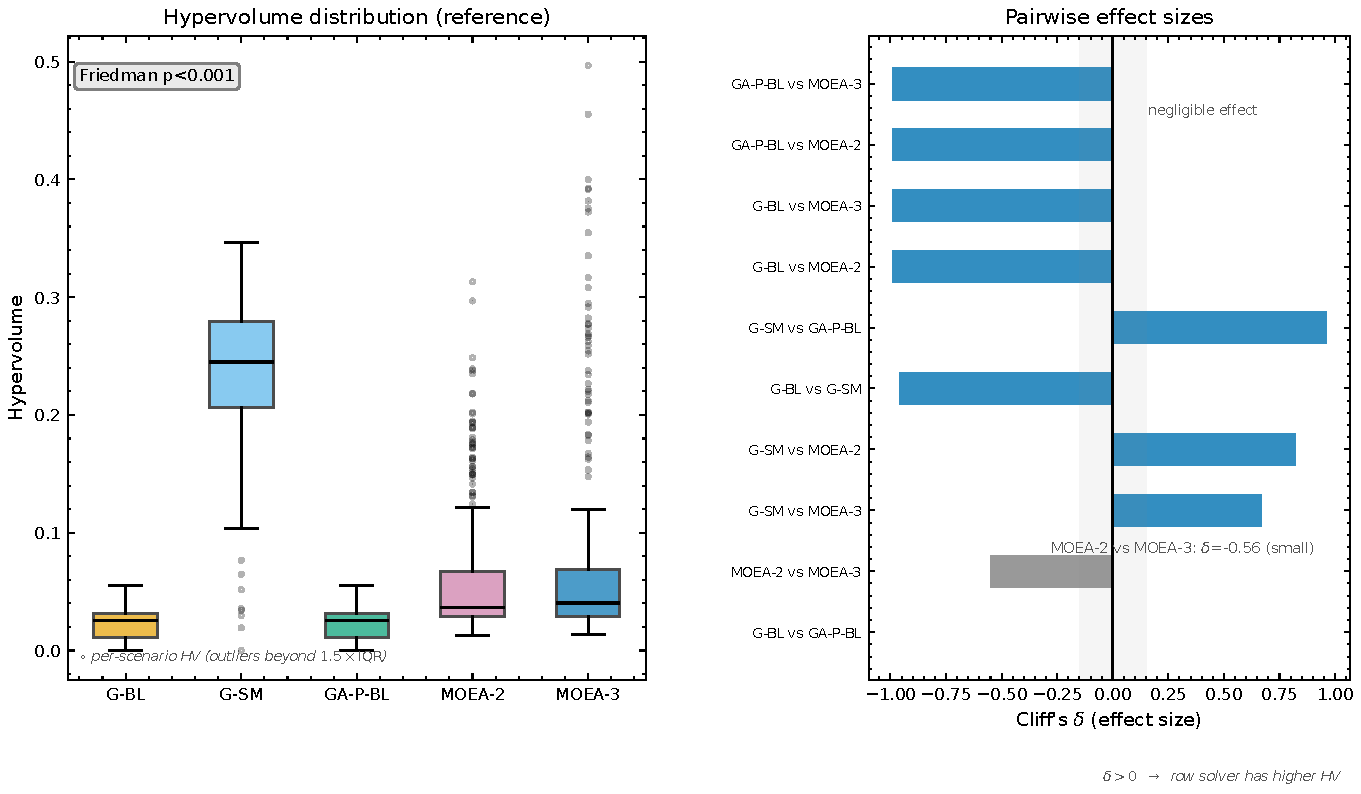
\includegraphics[width=\textwidth]{fig1_hypervolume.pdf}
    \caption{Statistical validation: (left) hypervolume distribution; (right) pairwise effect sizes as the matched-pairs sign statistic $\delta_{\text{pairs}} = (W-L)/n$, which equals Cliff's $\delta$ for the within-scenario pairing; the gray band marks the negligible-effect range ($|\delta|<0.147$ of \citet{Romano2006}; the conventional unpaired $\delta$ is weaker for the within-pair comparisons, see \S\ref{sec:evaluation-metrics}).}
    \label{fig:fig1}
\end{figure}

Fig.~\ref{fig:fig1} summarizes the statistical evidence behind these
comparisons. The left panel shows the per-scenario hypervolume (HV)
distribution of each solver under a shared min--max normalization: the
multi-point NSGA-III solvers attain higher pooled HV than G-BL, while the
extreme operating point of G-SM yields an HV comparable to the NSGA-III
variants. The right panel reports pairwise effect sizes on
HV as the matched-pairs sign statistic; bars outside the gray band ($|\delta|<0.147$) exceed the negligible-effect
threshold, and the direction convention is that positive $\delta$ favors the
row solver. Because HV rewards front cardinality as well as front quality,
these rankings are interpreted only as secondary diagnostics --- the
point-count confound is analyzed in \S~\ref{sec:pareto-coupling}.

The following sections deepen this overall analysis from five perspectives:
\S\ref{sec:squint-special} examines the special trade-off of squint-aware scheduling,
\S\ref{sec:scale-sensitivity} investigates scale sensitivity (how multi-objective advantage varies with target density),
\S\ref{sec:pareto-coupling} reveals the geometric mechanism of Pareto compression,
\S\ref{sec:ablation} verifies the condition dependence of this mechanism through ablation,
and \S\ref{sec:robustness-calibration} separates initialization and search-budget confounds through robustness controls.

% ── 6.2 Squint-Aware Special Regime ──
\subsection{Squint-Aware Special Regime}
\label{sec:squint-special}
The squint-minimized greedy solver (G-SM) improves NESZ radiometric quality ($f_3$)
relative to the profit-only baseline (G-BL) by selecting observation times that
minimize squint angle within each visibility window.
Across all 200 scenarios, this produces a large positive effect on $f_3$
(Cliff's $\delta = +0.99$, $p \approx 1.5\times10^{-34}$, on a per-scenario
paired basis: 199 of 200 scenarios improve) at a substantial aggregate cost
in coverage (Cliff's $\delta = -1.0$, $p < 10^{-34}$, on $f_1^*$; raw $f_1$ is used here because G-BL yields constant $f_1^* = 1.0$ by definition, for which the normalized-profit comparison degenerates to a one-sample test against a fixed value).
The trade-off, however, is strongly density-dependent.
In sparse scenarios (S1, $N = 20$), G-SM drops to $f_1^* = 0.51 \pm 0.16$
($-49\%$ vs.\ G-BL at $1.00$) while improving $f_3$ from $0.497 \pm 0.044$ to
$0.722 \pm 0.058$ ($+45\%$).
In dense scenarios (S4, $N = 500$), the $f_1$ cost escalates:
G-SM achieves $f_1^* = 0.37 \pm 0.12$ ($-63\%$), with $f_3$ rising from
$0.675 \pm 0.074$ to $0.786 \pm 0.046$ ($+16\%$).
Fig.~\ref{fig:fig2} visualizes this density-dependent trade-off: the
Locally Estimated Scatterplot Smoothing (LOESS)
trend in panel (c) identifies a transition region around $N = 100$
where the $f_1$ penalty grows rapidly.
The radiometric advantage narrows with density ($+45\%$ at S1 to
$+16\%$ at S4) as tightly packed time windows constrain how far each
acquisition can be moved toward the squint-minimizing time, while the
coverage cost remains large at every density (G-SM schedules, on average,
$44\%$ of the tasks G-BL selects at S1, falling to $\sim$20--27\% at
$N \geq 100$; these are means of the per-scenario scheduled-task-count
ratios, the profit-side analogue of which appears in
Table~\ref{tab:solver-profiles}).
\begin{figure}[H]
    \centering
    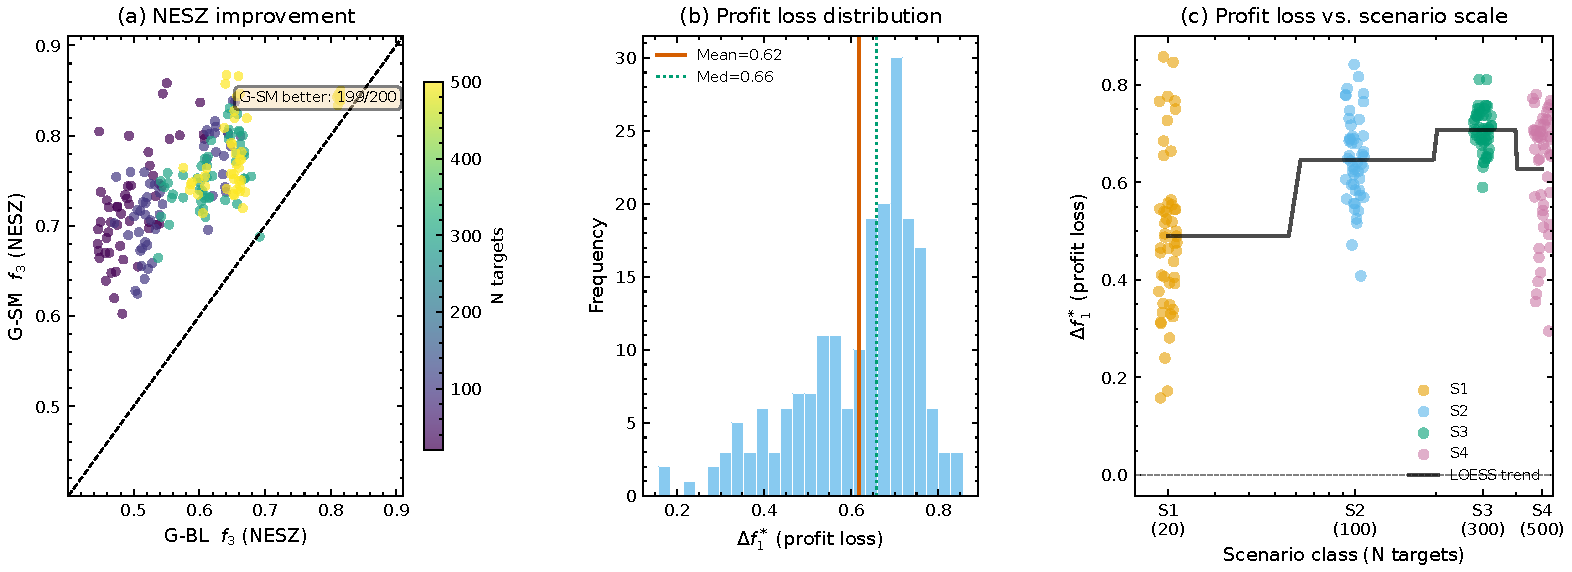
\includegraphics[width=\textwidth]{fig2_squint_effect.pdf}
    \caption{Effect of squint-aware scheduling: (a) $f_3$ scatter; (b) $\Delta f_1^*$ histogram; (c) $\Delta f_1^*$ vs.\ $N$ with LOESS trend}
    \label{fig:fig2}
\end{figure}

% ── 6.3 Scale Sensitivity (Fig 5) ──
\subsection{Scale Sensitivity}
\label{sec:scale-sensitivity}
The gap between MOEA-2 and G-BL varies systematically with scenario density
(Fig.~\ref{fig:fig3}, Table~\ref{tab:scale-sensitivity}).
MOEA-2's coverage deficit relative to G-BL is confined to sparse densities:
from $f_1^* = 0.86 \pm 0.14$ at S1 ($N = 20$) it rises to
$0.985 \pm 0.03$ at S2 ($N = 100$), and reaches $0.996$--$0.999$ at
$N \geq 150$ (S7--S8, S3), remaining within $1\%$ of G-BL at S4 ($0.996$).
The $f_2$ improvement over G-BL follows the same contraction, falling from $+33.7\%$ (S1)
to $+3.5\%$ (S2) and to $+1.3\%$ or less at $N \geq 150$.
The proportion of scenarios where MOEA-2's coverage falls measurably short of
G-BL ($f_1^* < 0.95$, i.e., a coverage deficit exceeding 5\%)
collapses from $80\%$ (S1) to $10\%$ (S2) and to $0\%$ at $N \geq 150$.
The coverage cost of multi-objective optimization is therefore a sparse-density phenomenon:
between $N = 20$ and $N = 100$ the solver transitions from actively trading off
coverage for quality to operating at the greedy baseline, and beyond
$N = 150$ the deficit is effectively zero.
\begin{figure}[H]
    \centering
    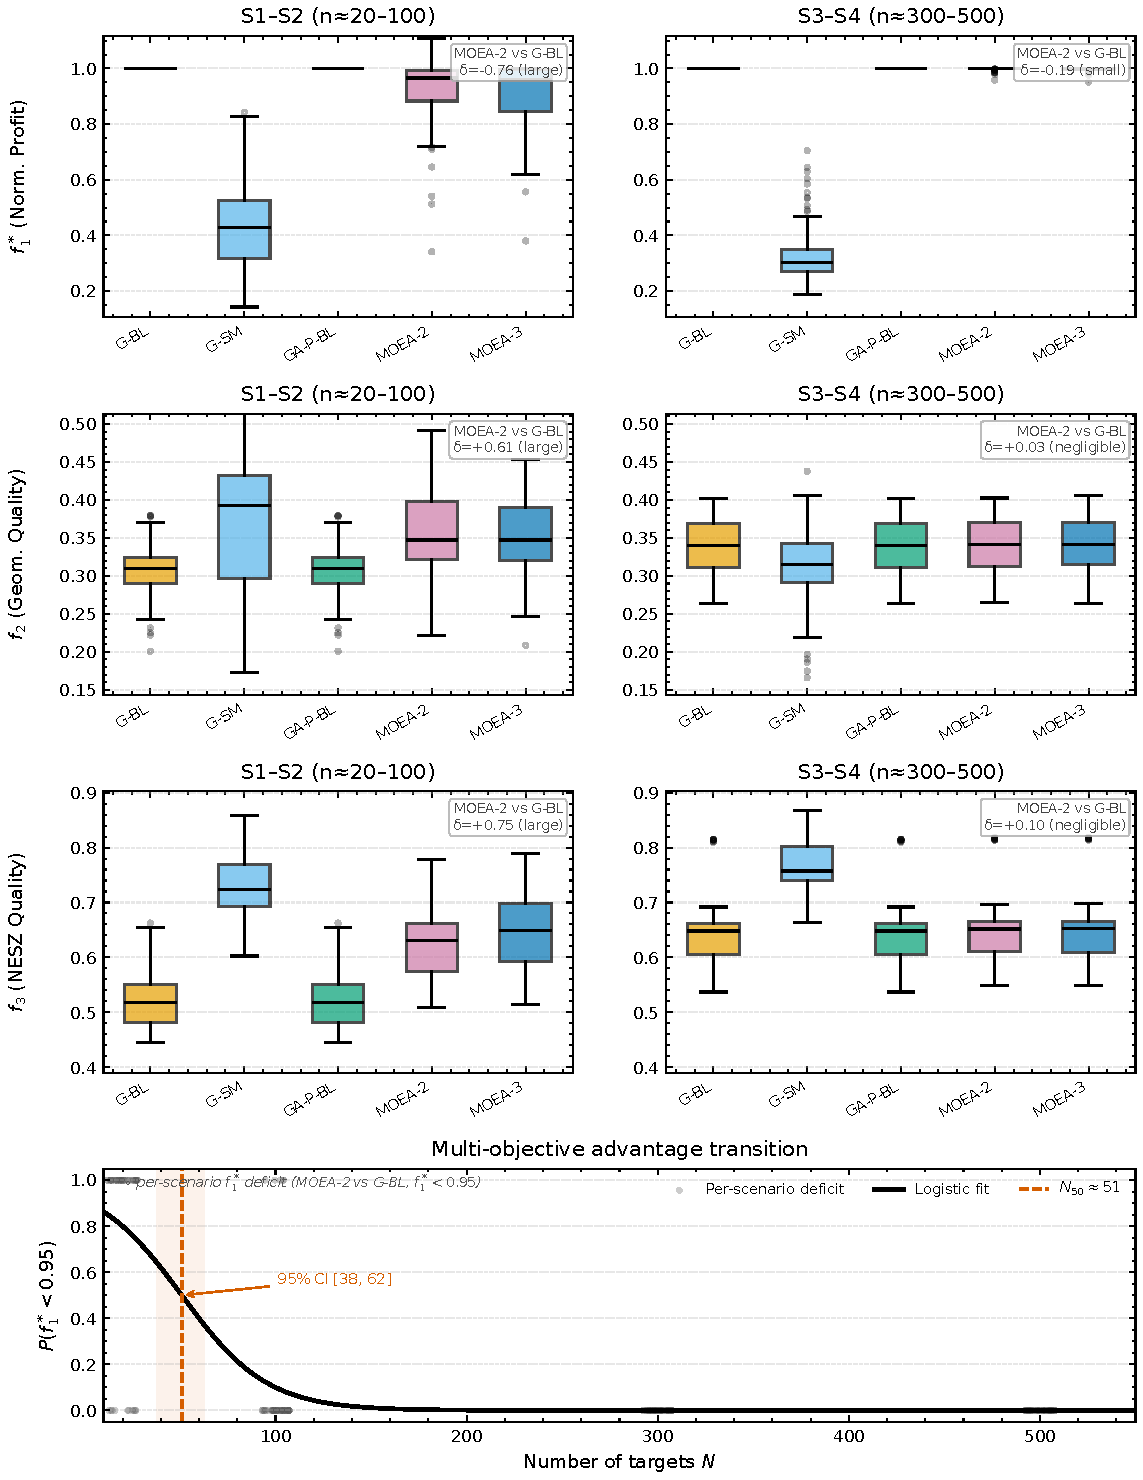
\includegraphics[width=0.75\textwidth]{fig3_scale_sensitivity.pdf}
    \caption{Scale sensitivity: (top) per-objective distributions of normalized profit $f_1^*$, geometric quality $f_2$, and radiometric quality $f_3$ for sparse (S1--S2) and dense (S3--S4) scenario classes; (bottom) logistic fit to the proportion of scenarios with a coverage deficit ($f_1^* < 0.95$), with jittered per-scenario indicators.}
    \label{fig:fig3}
\end{figure}
\begin{table}[H]
\centering
\caption{Scale sensitivity of MOEA-2 vs.\ G-BL. $f_2$ improvement is the mean of per-scenario ratios ($+34\%$ at S1 on this basis; the ratio of pooled means gives $+33\%$). S7 and S8 are intermediate scale points run for MOEA-2 and the two greedy baselines only (\S\ref{sec:experiment-design}); classes are ordered by target count $N$.}
\label{tab:scale-sensitivity}
\begin{tabular}{lcccc}
\toprule
\textbf{Class} & $N$ & $f_1^*$ (MOEA-2) & $f_2$ improvement & \% $f_1^* < 0.95$ \\
\midrule
S1 & 20   & $0.86 \pm 0.13$ & +33.7\% ($\pm 14.3$) & 80\% \\
S2 & 100  & $0.98 \pm 0.03$ & +3.6\% ($\pm 3.6$) & 10\% \\
S7 & 150  & $1.00 \pm 0.01$ & +1.3\% & 0\% \\
S8 & 200  & $1.00 \pm 0.00$ & +0.8\% & 0\% \\
S3 & 300  & $1.00 \pm 0.00$ & +0.4\% ($\pm 0.2$) & 0\% \\
S4 & 500  & $1.00 \pm 0.01$ & +0.3\% ($\pm 0.2$) & 0\% \\
\bottomrule
\end{tabular}
\end{table}
Fitting a logistic regression to the proportion of scenarios with
$f_1^* < 0.95$ across the six density points ($N=20, 100, 150, 200, 300, 500$)
yields a transition midpoint $N_{50} \approx 50$ targets. This estimate is
weakly constrained: only the two sparse densities ($N=20, 100$) carry
informative deficit proportions ($80\%$ and $10\%$), while the four denser
points are all at most $1\%$, so the bootstrap confidence interval is wide
($N_{50} \in [30, 62]$). $N_{50}$ should therefore be read as a coarse indicator that the
transition is confined to $N \in [20, 100]$, not as a precise threshold.
Beyond $N \approx 150$, no scenario shows a
coverage deficit exceeding $5\%$.
The transition between a measurable and a negligible multi-objective
advantage therefore lies in the $N \in [20, 100]$ band, and beyond $N = 150$
the advantage is effectively absent.
The $f_3$ row of Fig.~\ref{fig:fig3} shows the same pattern on the
radiometric objective: at sparse density MOEA-3 separates visibly from G-BL
and G-SM sits in its own high-$f_3$ regime, whereas the dense panels show all
solvers converging to nearly identical distributions, consistent with
Table~\ref{tab:solver-profiles}.

% ── 6.4 Mechanism of Pareto Compression ──
\subsection{Mechanism of Pareto Compression}\label{sec:pareto-coupling}

\textbf{Phenomenon 1: Front compression.}
Fig.~\ref{fig:fig4} visualizes the Pareto front on a representative S4
scenario. The front contains $4.7 \pm 4.4$ MOEA-3 non-dominated solutions
(MOEA-2: $1.6 \pm 0.9$) but is compressed: the found front spans only about
$0.08$ in $f_1^*$ and $0.014$ in $f_2$, against a total span of $\Delta f_2 \approx 0.14$
in sparse S1 scenarios, confirming the scale-dependent saturation documented
in \S\ref{sec:scale-sensitivity}. This compression is a property of the found
front under G-BL-seeded search rather than of the full feasible trade-off
surface: the squint-minimizing heuristic G-SM reaches feasible high-$f_3$
operating points ($f_3 \approx 0.79$ at S4, \S\ref{sec:squint-special}) outside
the MOEA-3 surface, so the dense-regime indistinguishability is established near the
full-coverage working point rather than over the entire feasible surface. In
dense regimes, solver convergence to
lower-squint geometries combined with schedule saturation limits quality
differentiation regardless of solver strategy. The MOEA-2 and MOEA-3 fronts
are nearly coincident at this density, indicating that adding $f_3$ as a third
objective produces little additional differentiation in the dense setting.

\begin{figure}[H]
    \centering
    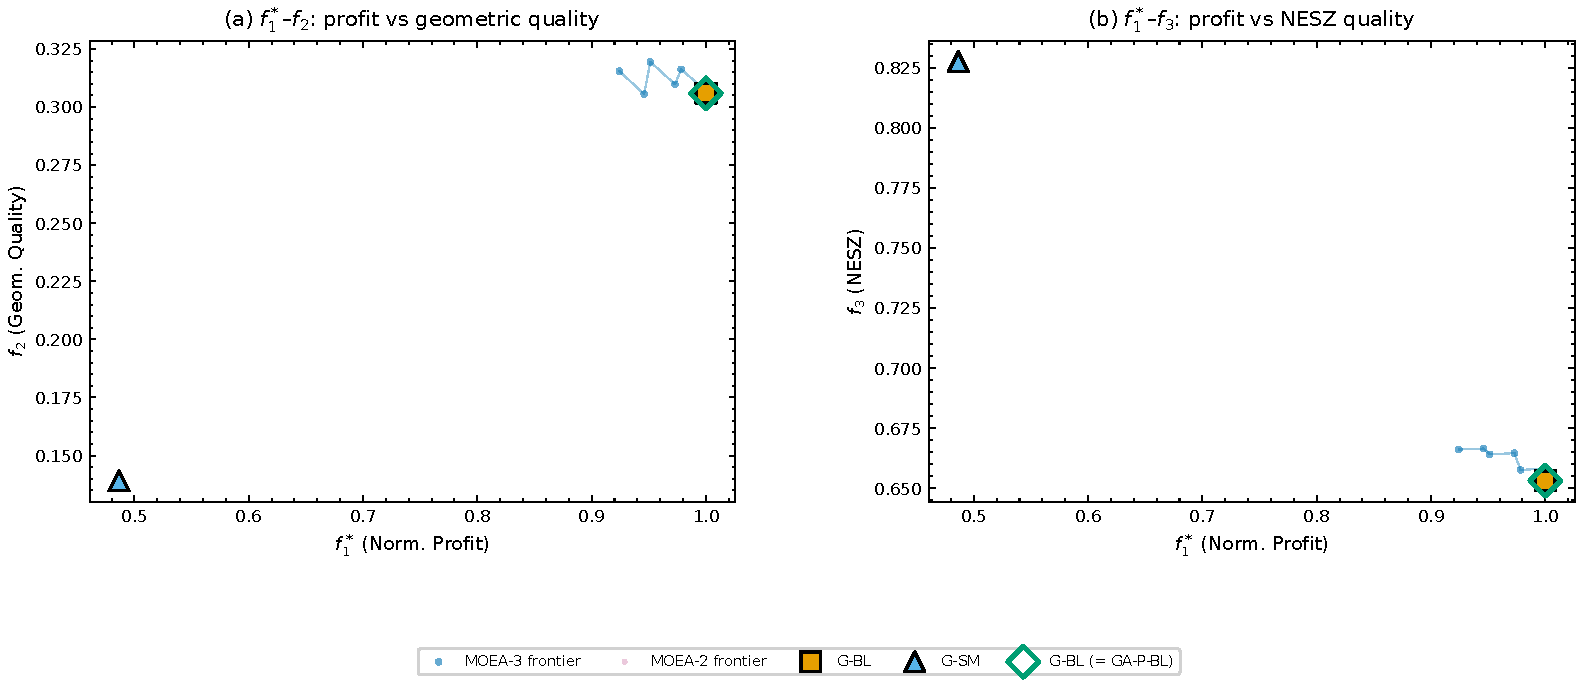
\includegraphics[width=0.75\textwidth]{fig4_pareto_front.pdf}
    \caption{Pareto front on a representative S4 scenario ($N=500$): MOEA-3 frontier with MOEA-2 overlay and baseline solver markers. Panel (a): $f_1^*$--$f_2$; panel (b): $f_1^*$--$f_3$.}
    \label{fig:fig4}
\end{figure}

The $f_1^*$--$f_2$ projection (panel a) shows an extremely compressed
surface: even for the S4 scenario with the widest $f_1^*$ spread, the
frontier spans only $f_1^* \in [0.92, 1.00]$ and $f_2 \in [0.306, 0.320]$
--- a near-vertical segment at full coverage.
Overlaying the single-point baseline solutions shows that G-BL sits at the
``full-coverage, moderate-quality'' corner of the frontier, while G-SM occupies
a qualitatively different region ($f_1^* \approx 0.37$, $f_3 \approx 0.79$) that
lies outside the MOEA-3 Pareto surface, a consequence of G-SM's aggressive
squint minimization.

\textbf{Phenomenon 2: Density-dependent third-objective value.}
The differentiation of MOEA-3 from MOEA-2 is density-dependent but modest:
at S1 the physics-aware solver attains $f_3 = 0.698\pm0.039$ versus
$0.657\pm0.040$ for MOEA-2 ($+6.2\%$ under the reported knee rules, paired
Wilcoxon $p = 5.5\times10^{-13}$; the matched-pairs sign statistic
is $+0.88$ on a per-scenario basis (47 of 50 scenarios), corresponding to a
conventional Cliff's $\delta$ of $+0.57$), at a
small $f_2$ cost ($0.376\pm0.050$ vs.\ $0.393\pm0.055$, $-4\%$, $p = 0.017$).
This margin is conditional on the knee-point rule: because MOEA-3's knee
maximizes $f_1+f_2+f_3$ while MOEA-2's knee maximizes $f_1+f_2$
(\S~\ref{sec:evaluation-metrics}), re-selecting both fronts under a matched
radiometric-aware rule gives a controlled third-objective margin of
$+4.9\%$ ($p = 2.3\times10^{-11}$, 47 of 50), whereas a radiometric-blind
rule gives $+0.05\%$ ($p = 0.86$); the headline comparison's remaining gap
thus conflates the objective function with knee selection, and the
objective itself contributes the $+4.9\%$ controlled margin that only
materializes under a radiometric-aware operating point.
This $+6.2\%$/$+4.9\%$ is robust to the reference-direction count: rerunning MOEA-3 at S1
with Das--Dennis $p=4$ ($H=15$, comparable in magnitude to MOEA-2's $H=13$ instead of the
default $H=91$) yields $f_3 = 0.702\pm0.041$ (50 scenarios, same pop=100,
gen=200, G-BL hot-start), statistically indistinguishable from the $p=12$
value $0.698$, so the third-objective gain is not an artifact of the
$7\times$ larger reference-direction set;
at S4 the means coincide ($0.680\pm0.073$ for both), though MOEA-3 retains a
modest per-scenario $f_3$ advantage (33 of 50, paired sign statistic
$+0.32$, $p = 4.5\times10^{-3}$; conventional Cliff's $\delta = +0.03$,
i.e.\ negligible in distribution although consistently signed). The third objective thus contributes a modest,
consistent $f_3$ gain at sparse density rather than a qualitatively distinct
regime: under the elevation-plane decomposition of \S\ref{sec:objective-functions},
MOEA-2 already attains high $f_3$ post-hoc, so the marginal value of explicitly
optimizing $f_3$ is bounded, and the principal quality contrast with the
profit-only baseline remains MOEA-3's $+40\%$ $f_3$ gain at S1. At operational
densities the advantage disappears because coverage pressure locks the
selection, not because the underlying $f_2$--$f_3$
trade-off vanishes---the within-schedule correlation remains negative but
is strongest at sparse density (about $-0.6$ to $-0.7$), settling to a
moderate $\approx -0.2$ to $-0.15$ at higher density
(\S\ref{sec:pareto-coupling}).

The HV ranking (Table~\ref{tab:hv}) differs from the coverage ranking (Table~\ref{tab:solver-profiles}): among the three tabulated solvers, G-BL ranks first in tabulated $f_1^*$ but third in HV, while the NSGA-III variants rank first and second in HV (MOEA-3, then MOEA-2), despite their lower coverage ranking. Notably, G-SM --- omitted from the
table because its single-point HV is dominated by point location rather than
front quality --- actually attains the highest HV of any solver ($0.2341$)
from its low-coverage, high-$f_3$ operating point
($f_1^* \approx 0.37$, $f_3 \approx 0.79$ at S4), so the HV ranking would
invert if it were included. This is precisely the point-count confound: HV
rewards an extreme single point more than a dense front near full coverage.
One sparse-density MOEA solution exceeds $f_1^*=1.00$ (one of 200 scenarios, $+10.8\%$ above G-BL), so G-BL is a near-optimal rather than a strict coverage anchor. This reversal is driven by point-count asymmetry: single-objective solvers contribute one point each to the HV reference set, while MOEA-3 contributes $33.8 \pm 8.4$ non-dominated points at S1 (MOEA-2: $6.8 \pm 2.1$), a cardinality gap that persists, less severely, at S3--S4. HV therefore conflates front quality with front cardinality, and the ranking should not be interpreted as a standalone quality judgment. The core phenomenon---front compression---is independent of HV ranking.

\textbf{Mechanism: geometric coupling and lower-squint convergence.}

Because $\theta$ and $\psi_{\text{sq}}$ are not independent but both
derived from the same LOS vector $\mathbf{l} = (l_x, l_y, l_z)$
(\S~\ref{sec:system-model}), the per-task $f_2$ and $f_3$ contributions
share geometric structure. To separate definitional coupling from
scheduler-induced correlation, we compute the analytical null
distribution by treating $\theta$ and $\psi_{\text{sq}}$ as independently
and uniformly distributed within
the accessible envelope ($\theta_{\text{elev}} \in [15^\circ, 50^\circ]$,
$|\psi_{\text{sq}}| \leq 45^\circ$, slightly wider than the C1 constraint
$[18^\circ, 47^\circ]$ to provide a conservative null baseline; the same
experimental squint envelope as \S\ref{sec:system-model}, not a specific
platform specification) and evaluating the Pearson correlation
of $f_{2,i} = \sin\theta_{\text{elev},i} \cos\psi_{\text{sq},i}$ and
$f_{3,i} = \cos^3\xi_i$ under independent angles.
Two independent baselines give the same order of magnitude: a permutation
null that independently shuffles the observed $\theta_{\text{elev}}$ and
$\psi_{\text{sq}}$ marginals within each density class gives
$r_{\text{null}} = -0.60$ (95\% spread $\pm 0.02$ across 20 shuffles per
class), and Monte Carlo sampling over the uniform box
$\theta_{\text{elev}} \in [16^\circ, 41^\circ]$,
$|\psi_{\text{sq}}| \leq 45^\circ$ gives $r_{\text{MC}} = -0.28$
($N_{\text{MC}} = 2\times 10^6$). We adopt the empirical-marginal
permutation value as the factorized null:
\begin{equation}
r_{\text{null}} = \frac{\mathrm{Cov}(f_2, f_3)}{\sqrt{\mathrm{Var}(f_2)\,\mathrm{Var}(f_3)}} \;\approx\; -0.60,
\label{eq:rnull}
\end{equation}
where the independence of $\theta_{\text{elev}}$ and $\psi_{\text{sq}}$ under the null
factorizes the moments, e.g., $E[f_2 f_3] = E[\sin\theta_{\text{elev}}\cos^3\theta_{\text{elev}}]\,E[\cos^4\psi_{\text{sq}}]$.
The \emph{negative} sign exposes a structural conflict, not redundancy:
in the $\theta_{\text{elev}}$-only limit (fixed squint), $f_{2,i} \propto \sin\theta_{\text{elev}}$ and
$f_{3,i} \propto \cos^3\theta_{\text{elev}}$ are strictly anti-monotonic
($r_\theta = -0.997$ in Monte Carlo), since $f_2$ favors high incidence while $f_3$
favors low incidence; in the $\psi_{\text{sq}}$-only limit (fixed
$\theta_{\text{elev}}$), both depend on $\cos\psi_{\text{sq}}$ positively
($r_\psi = +0.997$), since low squint improves both. The wide-envelope Monte
Carlo value ($-0.28$) is much weaker than the broadside limit because the
positive $\psi$-common-mode dilutes the $\theta_{\text{elev}}$ conflict.

\textit{Empirical correlation and lower-squint convergence.}
Pooled across all scheduled tasks from the 200 scenarios, the
per-task empirical correlation between $f_2$ and $f_3$ within the
solver-selected schedules is negative at every density, and it is
\emph{strongest at sparse density} rather than strengthening as density
rises: for the full-physics MOEA-3 (variant A) the pooled correlation is
$-0.63$ at S1 and falls to $-0.15$ (S2), $-0.13$ (S3), and $-0.23$ (S4).
Because the pooled statistic mixes between-schedule and within-schedule
variance, we also computed per-schedule correlations (Pearson $r$ within each
solver-selected schedule, one per scenario): the per-schedule
mean is $-0.72$ at S1 and $-0.15$/$-0.16$/$-0.18$ at S2/S3/S4
(Fisher-z means $-1.09$/$-0.16$/$-0.16$/$-0.19$, i.e.\ the mean of
$\mathrm{atanh}(r)$ over the 50 schedules per class), and individual
schedules span a wide range (S1 $r \in [-0.97, -0.03]$, entirely negative),
so the pooled value is representative but not uniform across schedules.
The $\theta_{\text{elev}}$-conflict therefore persists inside sparse schedules rather than being
reversed. All solvers select geometries shifted toward lower squint than the
visibility envelope (mean $|\psi_{\text{sq}}|$ $16$--$24^\circ$; \S\ref{sec:system-model}), and the
schedule correlation is strongly density-\emph{dependent}: at sparse density the
full-physics schedules match the factorized, independent-angle null
($-0.63$ versus $r_{\text{null}} \approx -0.60$), whereas at operational
density they weaken to about $-0.2$ to $-0.15$. The third objective's
class-mean indistinguishability at high density is therefore an
empirical convergence effect---not a mathematical identity between $f_2$
and $f_3$: a trace per-scenario $f_3$ advantage of MOEA-3 over MOEA-2
persists even at S4 (paired Wilcoxon $p = 4.5\times10^{-3}$, 33 of 50
scenarios), coexisting with negligible class-mean $f_3$ margins.

\textit{Envelope versus schedule correlation.}
Across the visibility-window grid (all window time-steps from 20 scenarios,
five per density class S1--S4 (seeds 0--4), at 10\,s resolution;
$7.6\times10^4$ geometry samples), evaluating the same objective
decomposition gives $\mathrm{corr}(f_2, f_3) \approx -0.36$ at every
density ($-0.35$ at S1 to $-0.37$ at S2--S3). This envelope value is
already weaker than the factorized null $r_{\text{null}} \approx -0.60$
(Eq.~\ref{eq:rnull}): real visibility geometry couples
$\theta_{\text{elev}}$ and $\psi_{\text{sq}}$ through the LOS vector (both
grow toward pass edges), adding a positive common-mode term that dilutes
the $\theta_{\text{elev}}$ conflict. The reported envelope therefore
spans squints only up to the C7 squint limit used at window generation
($|\psi_{\text{sq}}| \leq 45^\circ$); the scheduled geometries concentrate
at much smaller squints.

The solver-selected schedules move the correlation in opposite directions
at the two density regimes: at sparse density they restore the full
independent-angle conflict ($-0.63$, matching the $-0.60$ null)---the knee
solutions traverse the $\theta_{\text{elev}}$--$\xi$ trade-off across the
selected tasks instead of tracking the envelope's co-varying geometry; at
high density, coverage packing weakens the correlation below the
envelope value ($-0.15$ to $-0.23$). The sparse strengthening is an active
effect of the physical objectives, not of envelope geometry: the
visibility envelope alone supplies only the weaker $-0.36$ correlation.

Ablation studies identify which objective component drives this pattern.
Under variant B (squint removed from the objectives:
$f_2=\sin\theta_{\text{elev}}$, $f_3=\cos^3\theta_{\text{elev}}$ only), the
sparse schedule correlation collapses to $r = -0.23$, close to the
envelope value $-0.36$; under variant C (incidence removed: squint-only
objectives $f_2=\cos\psi_{\text{sq}}$, $f_3=\cos^3\psi_{\text{sq}}$) it
remains strong ($-0.65$), indistinguishable from the full-physics variant A
($-0.63$); under variant D (all physical objectives removed) it falls to
$-0.13$ at S1 and $-0.07$ at S2. The schedule-level conflict is thus
realized by any configuration that steers squint: variants that see
$\psi_{\text{sq}}$ (A and C) select configurations spanning the full
$\theta_{\text{elev}}$ trade-off, while variants blind to
$\psi_{\text{sq}}$ (B and D) produce schedules whose within-schedule
geometry sits at the weak envelope level. In the sparse regime the
squint-aware objectives thus retain solutions that traverse the
$f_2$--$f_3$ trade-off; without that steering the solver maximizes
coverage alone and temporal packing leaves the geometry near envelope
statistics. At higher density the full-physics residual correlation also
settles at a moderate level (about $-0.2$ to $-0.15$), so the ablation
contrast narrows; the third objective's value is lost not because the
conflict vanishes but because coverage pressure leaves no room to traverse
the trade-off and the $f_3$ margins between solvers become negligible.
A mechanical alternative---that the dense correlations weaken because the
realized $f_2$ value range compresses---is rejected by the data: the
pooled within-schedule $f_2$ standard deviation is effectively constant
across density classes ($0.16$ at S1--S3, $0.14$ at S4 for variant A;
pooled range $0.65$ in every class).
Consistent with this scale-dependent saturation, the per-density
hypervolume contracts at higher density: at S4 the pooled HV is
$0.25$ (MOEA-2) and $0.17$ (MOEA-3) of its S1 value, i.e. the S4/S1 HV
ratio is well below unity, reflecting the near-point front compression
documented in \S\ref{sec:pareto-coupling} (S4 fronts span only
$\Delta f_1^* \approx 0.06$) rather than a degradation of solution
quality.
We caution that the Pareto fronts reported here are best-known
approximations obtained via NSGA-III; whether they represent the
true Pareto-optimal set is unknown without exact methods, which remain
intractable for $N \geq 20$ in this problem class.

% ── 6.6 Ablation Study (physical modeling contribution) ──
\subsection{Ablation of Physical Modeling}
\label{sec:ablation}

To quantify the contribution of incidence-angle ($\theta$) and squint-angle
(${\psi_{\text{sq}}}$) modeling to solver performance, we repeat the MOEA-3
experiment with four objective-function variants:
%
\begin{description}
\item[A. Full physical (baseline)] $f_2 = \frac{1}{|\mathcal{S}|}\sum \sin\theta_i \cdot \cos\psi_i$,
      $f_3 = \frac{1}{|\mathcal{S}|}\sum \cos^3\theta_i \cdot \cos^3\psi_i$ (identical to the
      standard configuration in \S~\ref{sec:pareto-coupling}).
\item[B. No squint] $f_2 = \frac{1}{|\mathcal{S}|}\sum \sin\theta_i$,
      $f_3 = \frac{1}{|\mathcal{S}|}\sum \cos^3\theta_i$ (removes ${\psi_{\text{sq}}}$ component).
\item[C. No incidence] $f_2 = \frac{1}{|\mathcal{S}|}\sum \cos\psi_i$,
      $f_3 = \frac{1}{|\mathcal{S}|}\sum \cos^3\psi_i$ (removes $\theta$ component).
\item[D. No physics] $f_2 = f_3 = 1$ (constant per-task objective; solver receives
      no geometric information; $f_2$, $f_3$ shown in Table~\ref{tab:ablation} are post-hoc diagnostics
      computed from the actual observation geometry of the resulting schedule).
      Variant D serves as a null-model control: it tests whether the NSGA-III
      solver's performance is attributable to the physical content of $f_2$
      and $f_3$, or merely to the presence of additional objectives that
      structure the search.
\end{description}
%
All four variants use identical NSGA-III parameters (population $= 100$,
generations $= 200$, Das-Dennis $n=12$), the same 200 scenario files, and
the same G-BL hot-start injection. Only the objective functions differ,
making this a controlled ablation rather than a retuning experiment.
Within-solver ablation with identical NSGA-III parameters and the same
G-BL seed injection controls confounding factors sufficiently that the
Wilcoxon signed-rank test is appropriate for paired comparison of
objective-function variants.
Each variant completes 4 scenario classes $\times$ 50 seeds $= 200$ runs
(total: 800 runs across A--D). Degradation is reported as
$\Delta\% = (\text{A} - \text{V})/\text{A} \times 100$, where A is the full
physical baseline and V is the variant; negative values indicate the variant
outperforms the baseline on $f_1^*$.

\begin{table}[H]
\centering
\caption{Per-class ablation results. Bold: $p < 0.005$ (Wilcoxon signed-rank vs.~A; consistent with the Friedman--Wilcoxon framework of \S\ref{sec:scale-sensitivity}).}
\label{tab:ablation}
\begin{tabular}{llccccrc}
\toprule
\textbf{Class} & \textbf{V} & \textbf{$f_1^*$} & \textbf{$f_2$} &
\textbf{$f_3$} & \textbf{$f_1/n$} & \textbf{$n_\text{sel}$} &
\textbf{$\Delta f_1^*\%$} \\
\midrule
\multirow{4}{*}{S1 ($N=20$)}
 & A & $0.66 \pm 0.28$ & $0.569$ & $0.288$ & $5.93 \pm 1.10$ &
   $11.1 \pm 4.4$ & (baseline) \\
 & B & $0.72 \pm 0.33$ & $0.565$ & $0.281$ & $5.57 \pm 1.05$ &
   $12.8 \pm 5.5$ & $\mathbf{-10.0\%}$ \\
 & C & $0.51 \pm 0.22$ & $0.575$ & $0.300$ & $5.91 \pm 1.24$ &
   $8.8 \pm 3.5$ & $\mathbf{+21.6\%}$ \\
 & D & $0.81 \pm 0.34$ & $0.565$ & $0.266$ & $5.40 \pm 1.04$ &
   $14.7 \pm 5.6$ & $\mathbf{-23.5\%}$ \\
\midrule
\multirow{4}{*}{S2 ($N=100$)}
 & A & $0.86 \pm 0.39$ & $0.561$ & $0.245$ & $5.56 \pm 0.52$ &
   $47.6 \pm 21.4$ & (baseline) \\
 & B & $0.86 \pm 0.39$ & $0.560$ & $0.244$ & $5.55 \pm 0.56$ &
   $47.8 \pm 21.3$ & $+0.0\%$ \\
 & C & $0.83 \pm 0.37$ & $0.561$ & $0.247$ & $5.44 \pm 0.49$ &
   $46.6 \pm 20.0$ & $+3.5\%$ \\
 & D & $0.86 \pm 0.38$ & $0.561$ & $0.243$ & $5.46 \pm 0.60$ &
   $48.6 \pm 21.1$ & $-0.3\%$ \\
\midrule
\multirow{4}{*}{S3 ($N=300$)}
 & A & $0.97 \pm 0.25$ & $0.587$ & $0.175$ & $5.50 \pm 0.23$ &
   $151.1 \pm 38.7$ & (baseline) \\
 & B & $0.98 \pm 0.25$ & $0.587$ & $0.175$ & $5.52 \pm 0.23$ &
   $151.7 \pm 38.5$ & $-0.8\%$ \\
 & C & $0.98 \pm 0.25$ & $0.587$ & $0.175$ & $5.52 \pm 0.23$ &
   $151.1 \pm 38.3$ & $-0.3\%$ \\
 & D & $0.97 \pm 0.25$ & $0.587$ & $0.175$ & $5.51 \pm 0.22$ &
   $151.1 \pm 38.8$ & $-0.2\%$ \\
\midrule
\multirow{4}{*}{S4 ($N=500$)}
 & A & $0.97 \pm 0.28$ & $0.589$ & $0.170$ & $5.51 \pm 0.20$ &
   $190.2 \pm 56.2$ & (baseline) \\
 & B & $0.97 \pm 0.29$ & $0.589$ & $0.169$ & $5.50 \pm 0.19$ &
   $190.6 \pm 56.4$ & $-0.1\%$ \\
 & C & $0.97 \pm 0.28$ & $0.589$ & $0.170$ & $5.51 \pm 0.21$ &
   $191.0 \pm 55.8$ & $-0.4\%$ \\
 & D & $0.96 \pm 0.28$ & $0.589$ & $0.169$ & $5.50 \pm 0.19$ &
   $190.3 \pm 55.6$ & $+0.1\%$ \\
\bottomrule
\end{tabular}
\end{table}

\begin{figure}[H]
    \centering
    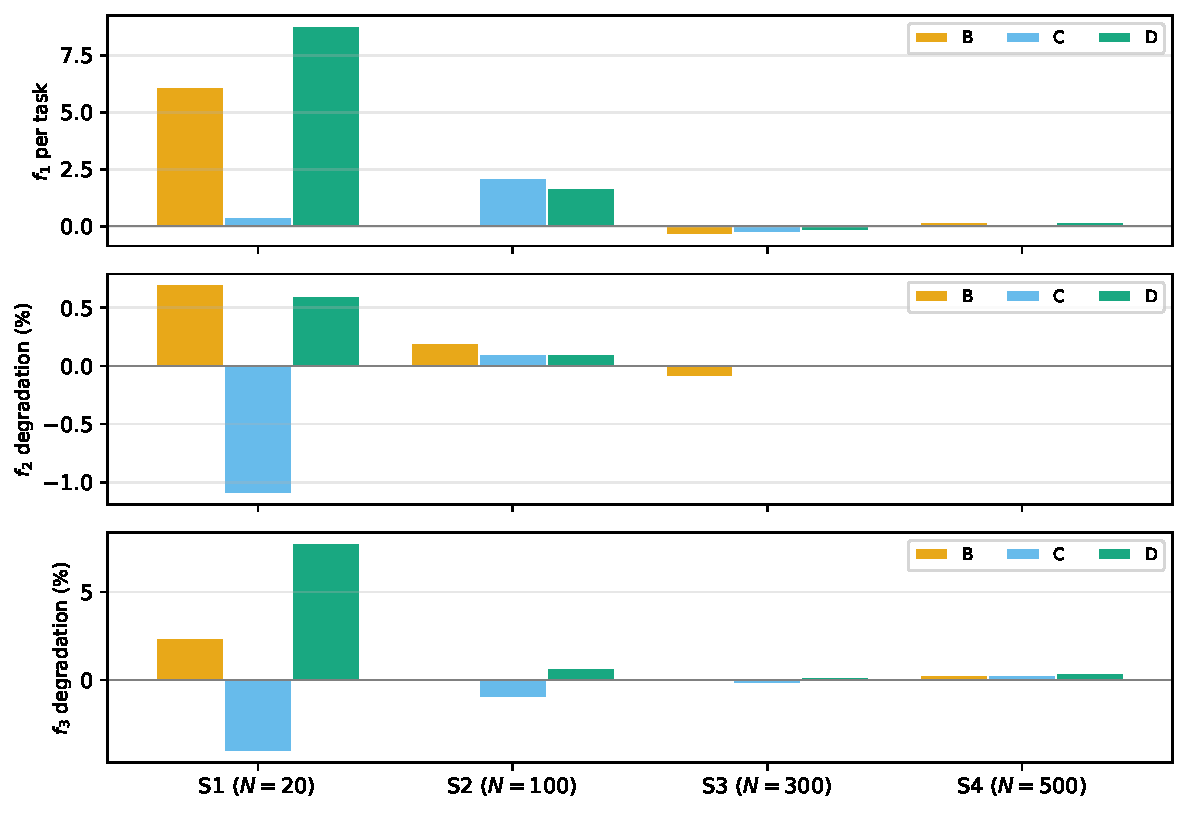
\includegraphics[width=\textwidth]{fig6_ablation.pdf}
    \caption{Ablation results across four objective-function variants (A--D) and four scenario classes}
    \label{fig:fig6}
\end{figure}

The ablation results in Table~\ref{tab:ablation} reveal that the influence
of physical objective modeling is concentrated in sparse scenarios and
vanishes as scenario density increases --- a pattern consistent with our
scale-sensitivity analysis (\S~\ref{sec:scale-sensitivity}).

At S1 ($N = 20$), all three ablations produce statistically
significant deviations. Variant C (no incidence) degrades $f_1^*$ by
$+21.6\%$ ($p = 1.9 \times 10^{-5}$), indicating that removing the
incidence-angle component from the objective function forces the solver
into poorer coverage outcomes. Conversely, variant D (no physics)
\emph{improves} apparent $f_1^*$ by $-23.5\%$ ($p = 1.4 \times 10^{-7}$)
by selecting $+32.4\%$ more tasks (14.7 vs.\ 11.1) --- the solver, freed
from geometric quality objectives, converges on raw profit maximization
at the cost of imaging quality. Variant B (no squint) also shows a
significant $-10.0\%$ improvement ($p = 8.0 \times 10^{-5}$),
consistent with the interpretation that removing $\psi_{\text{sq}}$
relaxes the geometric coupling that constrains task selection.

By S2 ($N = 100$), none of the three ablations reaches statistical
significance at $p < 0.005$. The $f_1^*$ of all variants falls within
$\pm 4\%$ of the baseline, and the per-task $f_1$ ($5.44$--$5.56$) and
$n_{\text{sel}}$ ($46.6$--$48.6$) are indistinguishable. The signal from
physical modeling has weakened to the point where it no longer produces
systematic coverage differences.

At S3--S4 ($N \geq 300$), every variant converges to within $1\%$ of the
baseline for $f_1^*$ and to within $0.5\%$ for $f_2$, $f_3$, and $n_{\text{sel}}$.
The per-task quality metrics ($f_1/n$) are identical to two decimal places
($5.50$--$5.52$) across all variants and scene classes. The $f_2$ value
is locked at $0.587$--$0.589$, varying by less than $0.3\%$. This numerical
invariance is the direct signature of the geometric upper bound discussed
in \S~\ref{sec:scale-sensitivity}: once the density of candidate observation
windows saturates the schedule ($N$ exceeds the maximum selectable
targets under the attitude maneuver and squint constraints), the
objective function only penalizes infeasible solutions rather than
differentiating among feasible ones. In this regime, the NSGA-III solver
acts as a constraint-filtered profit maximizer regardless of whether
$f_2$ and $f_3$ carry geometric meaning (A) or serve as constant
placeholders (D).

To verify that the convergence of Variants A and D is not an artifact
of insufficient solver convergence, we ran a control across 5 S3
($N = 300$) and 5 S4 ($N = 500$) scenarios with doubled population
($200$) and generation budget ($400$). Variant A (full physics)
achieves $f_1^* = 0.958 \pm 0.034$ (S3) and $0.892 \pm 0.025$ (S4);
Variant D (no physics) achieves $f_1^* = 0.963 \pm 0.020$ (S3) and
$0.890 \pm 0.026$ (S4), mean differences $\Delta f_1^* = -0.005$ (S3)
and $+0.002$ (S4), with post-hoc $f_2 \approx 0.595$ for both variants. The two variants remain
indistinguishable even with twice the computational budget across all
10 scenarios. Two interpretations are consistent
with this result: (i) the solver convergence to low-squint regimes,
where the empirical correlation $r = 0.93$--$0.98$ exceeds the
definitional null $r_{\text{null}} = -0.51$
(\S~\ref{sec:objective-functions}, Eq.~\ref{eq:rnull}) and aligns
$f_2$ with $f_3$, makes the physical objectives redundant once a
low-squint solution is selected; or (ii) NSGA-III cannot
differentiate between objectives at high density regardless of what
they encode (solver inadequacy). The control favors (i) --- doubling
the budget does not restore differentiation across 10 scenarios
(5 S3 + 5 S4), and a random-init Variant D control (no hot-start,
15 S3 + 15 S4 runs) still converges to low-squint
($f_2 = 0.605 \pm 0.003$, comparable to hot-start D's $0.594$), ruling
out hot-start residue as the sole driver --- but cannot fully rule out
(ii) without exact methods (documented intractable at $N \geq 20$ in
\S~\ref{sec:runtime}). We
therefore state the finding boundedly: under the tested
configuration, removing physical objectives produces
indistinguishable results, and the more parsimonious explanation is
solver convergence to a low-squint regime where the objectives
co-vary rather than mathematical irrelevance of the physical
objects.


% ── 6.6 Robustness and Calibration ──
\subsection{Robustness and Calibration}
\label{sec:robustness-calibration}
The mechanism above must be separated from initialization and search-budget
effects. We therefore use four control experiments.

\paragraph{Hot-start dependence.}
On 10 S1, 4 S2, 5 S3, and 5 S4 scenarios (3 seeds each), random-initialized MOEA-2 yields
$f_1^*$ deficits of approximately $-0.393 \pm 0.251$, $-0.551 \pm 0.060$, $-0.684 \pm 0.050$, and $-0.475 \pm 0.067$
(mean $\pm$ SD across runs) relative to hot-start MOEA-2, respectively. G-BL seeding therefore materially
improves coverage convergence at every tested density. The deficit peaks at
the dense S3 class ($-0.68$ at $N=300$), is smallest at the sparsest S1
($-0.39$ at $N=20$), and moderates at the densest S4 ($-0.48$ at
$N=500$), so high target density does not by itself make random initialization
sufficient. This constrains the
coverage-convergence claim: proximity to G-BL is initialization-dependent. The
initialization effect is not confined to coverage: random-init $f_2$ is
actually higher --- i.e.\ better geometric quality, under the convention of
Table~\ref{tab:solver-profiles} --- at sparse density ($0.505$ vs.\ $0.395$
at S1, $+28\%$; $0.460$ vs.\ $0.320$ at S2, $+44\%$), marginally higher at
S3 ($0.349$ vs.\ $0.339$, $+3\%$), and only lower at the densest S4
($0.347$ vs.\ $0.380$, $-9\%$). Random initialization therefore attains
comparable or better per-task geometric quality at S1--S3 at a large coverage
cost, and the G-BL anchor's material benefit lies in coverage, not geometry;
its geometric advantage is confined to the densest regime. The coverage
convergence is thus a G-BL
initialization effect rather than an artifact of the MOEA framework. Two caveats qualify this control: the
deficit sample is small (10/4/5/5 scenarios per class $\times$ 3 seeds, and 30
runs for the variant-D control, 15 per class), the scenarios were selected
as the first seeds of each density class in manifest order (subconfig A,
seeds 00 onward), the hot and random runs share
the same scenario seeds, so each deficit is a within-seed paired difference
rather than an independent-sample contrast, and the comparison is expressed
on the G-BL-normalized $f_1^*$ scale, on which the greedy anchor itself reads
exactly $1.0$ by construction; both argue for reading the deficit magnitudes
as indicative of the initialization effect rather than as precise coverage
bounds.

\paragraph{Perturbation sensitivity.}
A sweep over $\sigma\in\{0.1,0.3,0.5,0.7\}$ on MOEA-3 (10 S3 scenarios per
value, fixed solver seed) leaves mean $f_2$ and $f_3$ essentially unchanged
(mean $f_2 \approx 0.343$ and mean $f_3 \approx 0.610$ at every level, with
level-to-level variation of at most $\sim1\times10^{-3}$; MOEA-2 shows the
same flatness at $f_2 \approx 0.343$ and $f_3 \approx 0.609$), and coverage
stays flat at $200/300$ selected tasks (199.5 at $\sigma=0.7$). The per-task
$f_2$--$f_3$ coupling reported in \S~\ref{sec:pareto-coupling} is therefore a
property of the schedule geometry rather than of the perturbation magnitude,
and the indistinguishability persists across $\sigma=0.1$--$0.7$ rather than being a
byproduct of the $\sigma=0.5$ perturbation level. This sweep was run on
S3 scenarios only (the dense transition class); the perturbation flatness
is therefore directly established at high density and is not independently
assessed in sparse regimes. All control runs use the same Das--Dennis
partition ($p=12$, giving $H=91$ reference directions for three objectives
and $H=13$ for two) as the headline experiments.

\paragraph{Random-search calibration.}
On five S1 scenarios, 5,000 random task selections per scenario produce mean
$f_1^*=0.527\pm0.003$ and a 90th percentile of $0.930\pm0.008$; the best
sample reaches $1.000$ --- the G-BL profit, so random sampling never exceeded
the greedy baseline on these scenarios. Because the random sampler is
unconstrained and does not enforce C2--C4, this is an empirical bound on the
tested batch rather than a construction guarantee. High coverage under random
sampling therefore occurs only by chance; the MOEA's gains reflect structured
search.

\paragraph{Random-init control.}
A random-init variant-D control (15 S3 and 15 S4 runs, no G-BL hot start)
also converges to low squint, with $f_2=0.349\pm0.016$ at S3 and
$0.347\pm0.015$ at S4, statistically indistinguishable from the hot-started
D solver ($0.342\pm0.026$ at S3, $0.336\pm0.039$ at S4) on this per-task mean
at both densities. This $f_2$ agreement masks a coverage collapse: the
random-init D attains only $f_1^*=0.319\pm0.044$ and selects $70.3$ tasks at
S3 ($0.522\pm0.068$ and $117.8$ at S4), against near-full coverage for the
hot-started D, so the inference applies to the per-task geometric mean on
much smaller schedules rather than to coverage. The lower-squint convergence
is therefore objective-intrinsic rather than a hot-start
residue: the G-BL seed inserts tasks at their earliest feasible time and thus
biases hot-started runs toward the higher squint of the greedy schedule, most
visibly at high density. The A--D invariance itself already
holds at standard budget (Table~\ref{tab:ablation}: $\Delta f_1^* \leq
0.2\%$ at S3--S4), a physically forced consequence of coverage pressure
locking the selection at high density (\S~\ref{sec:pareto-coupling}); the
convergence is therefore not a budget artifact.

\paragraph{Search-budget control.}
To verify directly that the A--D invariance does not depend on the search
budget, we reran the full-physics (A) and no-physics (D) variants at double
budget (population 200, 400 generations) on five S3 and five S4 scenarios
under the current solver code. The A--D difference in $f_1^*$ remains
negligible ($-0.12\%$ at S3, $-0.44\%$ at S4; both variants reach full
coverage), corroborating the standard-budget ablation and confirming that
the invariance reflects coverage pressure at high density rather than the
budget expended. Quality is likewise budget-stable: comparing the
double-budget full-physics runs against the standard-budget runs on the
same ten scenarios shifts $f_1^*$ by only $-0.05\%$ (S3) and $-0.35\%$
(S4), $f_2$ by $+0.64\%$/$+0.52\%$, and $f_3$ by $+1.64\%$/$+0.97\%$
(all below $2\%$), so the reported sub-$2\%$ dense-regime quality margins
are not an artifact of premature convergence at the tested budget; a
convergence trace for the 200-generation frontier is not reported, and the
quality claims are understood as conditional on the tested budget.
These controls collectively favor the lower-squint convergence explanation
over hot-start residue, noise-level sensitivity, or random chance, while
not ruling out all algorithm-specific effects.

% ============================================================
%  7. DISCUSSION (~1200 words)
% ============================================================
\section{Discussion}
\subsection{Summary of Findings}
\label{sec:summary}
At
$N=20$ the three dimensions form a genuine trade-off
surface --- G-BL retains $f_1^* = 1.00$ at a moderate $f_3$
($0.497$), MOEA-2 reaches the highest $f_2$ ($0.393$) alongside a
$f_3$ of $0.657$, and MOEA-3 trades $f_2$ ($-4\%$ vs.\ MOEA-2) for the highest $f_3$
($0.698$, $+6.2\%$ vs.\ MOEA-2 under the reported knee rules) --- so no solver dominates on more than one
dimension, whereas at $N \geq 300$ all solvers converge to the G-BL anchor and
the greedy baseline is operationally sufficient.
Our experiment across 200 systematically varied scenarios yields five
interconnected findings:
\textbf{(1)}~the quality advantage of multi-objective optimization saturates with
target density ($+33.7\%$ in $f_2$ at $N=20$ falling to $+0.4\%$ at $N=500$);
\textbf{(2)}~the third objective is density-dependent rather than redundant:
per-task $f_2$--$f_3$ correlation within schedules stays negative at every
density, strongest at sparse density (about $-0.63$ pooled, $-0.72$
per-schedule, at S1 for the full-physics solver) and settling to a moderate
$\approx -0.2$ to $-0.15$ at higher density, and MOEA-3 separates from
MOEA-2 in $f_3$ at sparse
density ($+7\%$ at $N=20$) with the advantage shrinking to $\lesssim 0.2\%$
at $N \geq 300$, confirming the coverage-pressure mechanism detailed in
\S~\ref{sec:pareto-coupling}. Taken together, these results establish that
the Pareto front, while offering multiple quality-coverage configurations,
is compressed by the geometric coupling above: the narrow $f_2$ range limits
practical differentiation between solutions.
\textbf{(3)}~G-SM occupies a distinct high-radiometric-quality regime at
substantial density-dependent coverage cost;
\textbf{(4)}~solver outcomes become invariant to the choice of physical
objectives at $N \geq 300$ (ablation study); and
\textbf{(5)}~coverage convergence toward the G-BL anchor is conditional
on the hot start, not a structural property. The first four reflect
geometric properties of the single-pass observation geometry
(finding (2) being an empirical convergence effect under those
properties, \S~\ref{sec:pareto-coupling}); the fifth reflects solver
initialization.

The Friedman test on pooled HV confirms overall differences among the five
solvers across all 200 scenarios ($\chi^2=669.02$, $p<10^{-140}$; G-BL and
GA-P-BL coincide in 199 of 200 scenarios and never differ to GA-P-BL's
disadvantage, so the statistic is conservative toward fewer
distinct rankings). G-BL, GA-P-BL, and G-SM each contribute a single point
per scenario, so the pooled statistic is driven largely by the within-scenario
HV dispersion of the two multi-point NSGA-III solvers rather than by
baseline-vs-baseline differences. Pairwise Wilcoxon
signed-rank tests use the Bonferroni threshold $\alpha=0.005$
($\alpha=0.05/10$; the four-variant ablation of
\S~\ref{sec:ablation} applies $\alpha=0.05/12$ per density class); pairs
with zero within-pair difference are dropped from the Wilcoxon signed-rank
statistic and reported separately; interpretation
relies on Cliff's $\delta$ given the large sample size.
MOEA-2 and MOEA-3 differ on pooled HV with $\delta = -0.56$
($p < 10^{-5}$), but this contrast blends the sparse-regime divergence with
the dense-regime convergence and is inflated by the HV point-count
asymmetry (\S~\ref{sec:pareto-coupling}); contrasts involving
G-SM are large because it occupies an extreme radiometric-quality regime.

Independently of the multi-objective question, GA-P-BL output is numerically
identical to G-BL in 199 of 200 scenarios (never worse by construction),
because its never-worse-than-baseline guard
(Sec.~\ref{sec:ga-p-bl}) returns the greedy schedule on the single profit
objective; the present claims therefore concern the marginal value of adding
physical objectives rather than profit-oriented search alone.

\subsection{Operational Implications}
\label{sec:operational-implications}

The scale dependence has direct consequences for mission planning.
In sparse regimes ($N \leq 100$), MOEA-2 achieves a $+34\%$ geometric-quality
improvement at S1 at a $14\%$ coverage cost ($f_1^* = 0.86$
at $N=20$ relative to G-BL). Whether this trade-off is acceptable
depends on the application: for maritime surveillance, the
knee-point $+34\%$ $f_2$ gain at S1 corresponds to roughly a $25\%$ reduction in ground
pixel area (pixel area scales as $1/f_2$ for the geometric index of
Eq.~\ref{eq:f2}), and the coverage cost may be
justified; for area-monitoring missions, the greedy baseline remains
preferable. In dense regimes ($N \geq 300$), the multi-objective
advantage falls below $1\%$ improvement in $f_2$, while G-SM offers
the highest radiometric quality ($+16\%$ $f_3$ at S4) at a $63\%$
coverage cost; this gain comes from the one-line squint-minimization
heuristic rather than from multi-objective search.

The agility-envelope sensitivity, previously an open qualification, is
tested directly: repeating the sparse $N=20$ configurations with the
window-generation squint cap reduced from $45^\circ$ to $25^\circ$ and
$15^\circ$ (50 paired scenarios per cap, identical targets and seeds)
shows that the multi-objective edge contracts monotonically with the
envelope. Relative to G-BL in the same scenarios, MOEA-3's $f_2$
advantage shrinks from $+28\%$ at the $45^\circ$ cap to $+9\%$ at
$25^\circ$ and $+2.3\%$ at $15^\circ$, while its coverage cost shrinks
from $15\%$ to $4\%$ to $\approx 0\%$ ($f_1^* = 0.85$, $0.96$, $1.01$);
absolute geometry improves for every solver under the tighter cap
(G-BL $f_2$ rises from $0.295$ to $0.405$ to $0.448$), because window
filtering removes the low-quality high-squint options. The quality
advantage of physics-aware multi-objective scheduling is therefore
specific to wide-envelope platforms; on platforms with
$|\psi_{\text{sq}}| \lesssim 25^\circ$ agility---or without
Doppler-centroid compensation for large squints
(\S~\ref{sec:system-model})---the greedy baseline attains comparable
quality at full coverage even in sparse regimes. The logistic midpoint
$N_{50} \approx 50$ (\S~\ref{sec:scale-sensitivity}) provides a coarse
indicator between the density regimes. Our results suggest a conditional
operational guideline: for sparse observation requests ($N \lesssim 100$)
on squint-agile platforms (the $45^\circ$ experimental envelope of
\S\ref{sec:system-model}), MOEA-2 may provide geometric quality gains
that outweigh the coverage penalty in specific contexts---the knee point
trades $14\%$ coverage for $+33\%$ $f_2$, while the best-coverage front
point still gives $+12.5\%$ $f_2$ at zero coverage cost, a configuration
preferable when coverage cannot be sacrificed; for sparse requests on
narrow-envelope platforms, and for dense monitoring campaigns
($N \gtrsim 300$) on any platform, greedy methods (G-SM for radiometric
priority, G-BL for coverage priority) attain the tested family's coverage
reference and may be preferable. Indeed, the
MOEA-2 coverage gap relative to the coverage-only anchor is
$0\%$ at $N \geq 300$ (Table~\ref{tab:scale-sensitivity}); since GA-P-BL
output coincides with G-BL in 199 of 200 scenarios (and is never worse), no meaningful separate gap exists. The dense-regime greedy
choice also differs from quality steering on a timeliness dimension, by
construction rather than by a measured latency figure: G-BL places each
task at its earliest feasible time within the visibility window, whereas
quality-steering solutions may delay acquisitions to reach lower-squint
geometry, so the coverage-priority choice is the natural default when
acquisition timeliness matters.

\subsection{Transferability Across Remote-Sensing Domains}
The analytic device most likely to transfer beyond SAR is the
envelope--null--schedule decomposition of \S\ref{sec:pareto-coupling}: separating
the geometric correlation over the full feasible envelope from the
within-schedule residual isolates where an objective's value is lost to
saturation rather than to a mathematical redundancy. The geometric-resolution
objective ($f_2$) carries directly to optical systems, where ground sample
distance grows with off-nadir angle (the optical pixel footprint scales
as $1/\cos^2\eta$), and the same density-dependent
saturation would appear; the radiometric objective ($f_3$, NESZ) does not,
because optical radiometry depends on illumination and cloud cover rather
than on observation geometry alone. The decomposition, rather than any
single solver ranking, is the transferable contribution.

% ── 7.4 Limitations ──
\subsection{Limitations}\label{sec:limitations}
Our study is bounded by scope decisions that define directions for future work.
The density-dependent third-objective indistinguishability reported above is specific to the single-pass,
single-satellite Stripmap setting: it reflects solver convergence to lower-squint
geometries that attenuate the envelope-level $f_2$--$f_3$ correlation while
the residual within-schedule $\theta$-conflict persists (negative at all
densities, strongest at sparse density; \S\ref{sec:pareto-coupling},
Eq.~\ref{eq:rnull}), not a mathematical
identity between $f_2$ and $f_3$. In multi-pass or multi-satellite
settings with greater angular diversity, the $\theta$-conflict would
re-emerge and the third objective may become discriminative; the static,
advance-known target set likewise excludes dynamic arrivals and
rolling-horizon re-optimization, where newly arriving tasks compete
within the same windows and could shift the saturation threshold. Similarly,
ScanSAR, Spotlight, and TOPS modes introduce different NESZ and resolution
dependencies beyond Stripmap, and the scenario design uses a fixed orbit
(693 km circular LEO) without exploring sensitivity to orbital parameters.
The hot-start control experiment
(\S~\ref{sec:robustness-calibration}) indicates that G-BL
initialization materially improves MOEA convergence; the coverage
convergence reported here is conditional on this initialization, and
full-scale random-init experiments are needed to establish the unconditional
behavior. The hot-start dependence implies that the coverage-convergence result
reflects the combination of G-BL prior knowledge with MOEA search; whether
the MOEA can independently discover high-coverage solutions without greedy
seeding remains an open question. Similarly, the NSGA-III
crowding-distance explanation for the S1 variant-D reversal
(\S~\ref{sec:ablation}) awaits verification with alternative crowding
operators. Two further scope notes bound the operational reading: the energy
and memory budgets (C3--C4) are deliberately set far below their caps, so the
saturation result holds in the resource-unconstrained regime and may not
transfer when energy or downlink capacity is the binding constraint; and the
dwell time is fixed at 30\,s, removing the dwell-versus-SNR trade-off that an
agile scheduler could otherwise exploit. The utility model also optimizes quality
and quantity at a fixed timeliness operating point without an explicit
latency or urgency objective; the time-critical monitoring motivation of
\S~\ref{sec:introduction} is therefore addressed only indirectly, through
the earliest-feasible placement of the greedy baseline and the short dwell
interval, rather than as a distinct scheduling dimension. The reference-point counts of MOEA-2
($H=13$) and MOEA-3 ($H=91$) differ by construction, but a matched control at $p=4$
($H=15$, \S~\ref{sec:pareto-coupling}) confirms the sparse-regime $f_3$ gain is not driven by
reference-direction density. Finally, we do not benchmark against learning-based
schedulers (e.g., \citet{Chen2025NeuralPriority}), which represent an alternative
methodological family; a systematic comparison of physics-aware
heuristic methods against data-driven approaches is left to
future work.
% ============================================================
%  8. CONCLUSION (~250 words)
% ============================================================
\section{Conclusion}
We described a physics-aware multi-objective optimization approach for
agile SAR satellite scheduling that integrates NESZ radiometric quality
and geometric resolution as explicit optimization objectives alongside
coverage profit.
Five configurations (two greedy heuristics, a single-objective GA control
numerically identical to G-BL in 199 of 200 scenarios, and NSGA-III with two and three objectives) were
compared on
200 systematically varied scenarios across four density classes.
The central finding is a scale-dependent empirical saturation of the marginal
benefit of physical objectives in G-BL-seeded MOEA formulations for
single-pass, single-satellite Stripmap SAR operations under the tested
configuration.
At sparse density the three objectives form a genuine trade-off surface
(MOEA-2 raises $f_2$ by $+34\%$ (knee-point value; best-coverage front $+12.5\%$) and MOEA-3 raises $f_3$ by $+40\%$ over the
greedy anchor at a $14$--$15\%$ coverage cost), while at high densities the marginal quality
gains become negligible and all configurations converge to the G-BL
reference.
The saturation arises from solver convergence to lower-squint regimes under
which the geometric coupling aligns $f_2$ and $f_3$ along the shared
$\cos\psi_{\text{sq}}$ factor, making the third objective indistinguishable
from the two-objective formulation at high densities under the tested
search, not at sparse density; this is a convergence effect, and the reported
fronts are best-known NSGA-III approximations rather than verified Pareto sets.
Coverage convergence toward
the G-BL reference is conditional on the hot start; the geometric coupling
(visibility-envelope correlation $-0.36$, restored to the independent-angle
null strength of $-0.60$ in sparse schedules at $-0.63$, and collapsing to
$-0.2$ to $-0.15$ at high density within schedules) is the
anchor-independent result (\S~\ref{sec:pareto-coupling}).
GA-P-BL output coincides with the G-BL reference in 199 of 200 scenarios,
because its never-worse-than-baseline
guard triggers on the single profit objective in every scenario but one, so this result
delimits the benefit of adding physical objectives.
This saturation regime applies to the evaluated target-density range ($N=20$--$500$)
and G-BL-seeded NSGA-III search.
For mission planning, the operational implication is conditional:
multi-objective optimization provides measurable benefit only when
observation requests are sparse; at dense monitoring cadences, greedy
methods attain the tested family's coverage reference. These findings establish an
empirical, conditional saturation regime for what physics-aware multi-objective scheduling can
contribute to single-satellite SAR operations, and provide a baseline
against which multi-satellite, multi-pass, and multi-mode extensions
can be measured.
% ── AI and AI-Assisted Technologies (Elsevier/ASR policy) ──
\section*{Declaration of generative AI and AI-assisted technologies in the manuscript preparation process}
During the preparation of this work the author used AI-assisted
tools (Claude, Codex) for manuscript preparation and revision
assistance only. The author reviewed and edited all
AI-assisted output and takes full responsibility for the content
of this article.
% ── Acknowledgments ──
\section*{Acknowledgments}
The author thanks Prof.\ LIU Fanming (Harbin Engineering University) for
guidance and support throughout this research. Prof.\ Liu is a co-author of
\citet{Wu2026WhaleHighDensity}; his contribution to the present work was limited
to advisory discussions on research direction and did not include experimental
design, data analysis, or manuscript preparation.
% ── CRediT Authorship Contribution Statement ──
\section*{CRediT Authorship Contribution Statement}
\textbf{Liu Shuhao:} Conceptualization, Methodology, Software, Validation,
Formal Analysis, Investigation, Resources, Data Curation,
Writing -- Original Draft, Writing -- Review \& Editing, Visualization.
% ── Data Availability Statement ──
\section*{Data Availability Statement}
Solver code (NSGA-III via \texttt{pymoo} 0.6.1.6), scenario generators, fixed seeds and configurations, processed
JSON/CSV results, analysis scripts, and figures are available from the
corresponding author. The companion repository is publicly available at
\url{https://github.com/liushuhao/sar-quality-aware-scheduling}.
Generated binary scenario files and per-run pickle objects are not
tracked; they can be regenerated using the supplied scripts.
% ── Declaration of Competing Interest (Elsevier requirement) ──
\section*{Declaration of Competing Interest}
The author declares that he has no known competing financial interests or
personal relationships that could have appeared to influence the work
reported in this paper.
% ── Funding (Elsevier requirement) ──
\section*{Funding}
This research received no specific grant from any funding agency in the
public, commercial, or not-for-profit sectors. The work was performed as
part of the author's doctoral studies at Harbin Engineering University,
College of Intelligent Systems Science and Engineering.
% ═══════════════════════════════════════════════════
%  BIBLIOGRAPHY
% ═══════════════════════════════════════════════════
\bibliographystyle{elsarticle-harv}
\bibliography{small-paper-ijae}
\end{document}
